\documentclass{article}
\usepackage[utf8]{inputenc}
\usepackage{graphicx}
\usepackage{amsmath}
\usepackage{amssymb}
\usepackage{amsfonts}
\usepackage{indentfirst}
\usepackage{gensymb}
\usepackage[a4paper, total={7in, 10in}]{geometry}
\graphicspath{ {./../res/} }
\numberwithin{equation}{section}

\title{Optical Mie resonances in high-refractive-index nanostructures}
\author{Neven Gentil}
\date{April 2022}

\begin{document}

\maketitle

\twocolumn

\section{Theory}

The first step is to produce a theorical support in order to experimentally check the simulation created on these equations. More precisely, we will mathematicaly represent our nanostructure and extract measurable factors from this.

\subsection{Vector Spherical Harmonics}

First at all, let's describe the general composition of our problem: given a spherical particle of radius $a$ droped in a certain medium, we hit it with a monochromatic light. With a fixed refractive index $N$ for the nanosphere, respectively $N_{I}$ for the medium and other specifics parameters for electromagnetic materials like the permeability $\mu$, our objective is to, theoretically, compute the electromagnetic field for the medium surrounding the particle and inside this particle itself, in order to find the expression of the scattered light.

Let's start with an arbitrary electromagnetic field represented by the couple of \textit{monochromatic} vector field $(\textbf{E}, \textbf{H})$ which satisfies the Maxwell equations:
\begin{align}
\nabla \cdot \textbf{E} &= 0\\
\nabla \cdot \textbf{H} &= 0\\
\nabla \times \textbf{E} &= i\omega \mu \textbf{H} \label{eq:rot_e} \\
\nabla \times \textbf{H} &= -i\omega \epsilon \textbf{E} \label{eq:rot_h}
\end{align}
Given the relation $k^{2} = \omega ^{2}\epsilon \mu$ and standards formula from vectorial analysis, we obtain a couple of \textit{vector wave equation}:
\begin{align}
\nabla ^{2} \textbf{E} + k^{2}\textbf{E}&=0\\
\nabla ^{2} \textbf{H} + k^{2}\textbf{H}&=0
\end{align}
where $\nabla ^{2}$ is the vector Laplace operator.

An important thing to notice is that any vector field with zero divergence and satisfying the vector wave equation is a valid electric/magnetic field where we can obtain the corresponding magnetic/electric field by the curl (\ref{eq:rot_e})/(\ref{eq:rot_h}).

In this way, it is possible to create a vector function $\textbf{M}$ depending on a scalar function $\psi$ and an arbitrary constant vector $\textbf{c}$:
\begin{align}
\textbf{M} = \nabla \times (\textbf{c}\psi)
\end{align}
where \textbf{M} directly satisfies the condition $\nabla \cdot \textbf{M} = 0$. If we replace the expression of \textbf{M} in the vector wave equation, and thanks to (\ref{eq:rot_rot_a}), we easily obtain:
\begin{align}
\nabla ^{2} \textbf{M} + k^{2}\textbf{M} = \nabla \times [\textbf{c}(\nabla ^{2} \psi + k^{2}\psi)]
\end{align}
To satisfy the vector wave equation, $\psi$ should also satisfy the equivalent scalar wave equation:
\begin{align}\label{eq:psi_wave_eq}
\nabla ^{2} \psi + k^{2}\psi = 0
\end{align}
where, this time, $\nabla ^{2}$ is the scalar Laplace operator. By the way, if we denote $\nabla \times \textbf{N} = k \textbf{M}$, we have the perpendicular vector field of the artificial $M$, also satisfying the vector wave equation. Finally, we created the vector harmonics $\textbf{M}$ and $\textbf{N}$ with the scalar generating function $\psi$ associated to our initial electromagnetic field.

\subsection{Explicit Expansion Of Vector Spherical Harmonics}

The main idea to compute all solutions required is the following: given an incident electromagnetic field, we use the boundary conditions on the surface of our particle to get all fields resulting from interaction. Thereby, it could be interesting to use the spherical polar coordinates during the calculation and particularly to express the boundary conditions. That is why we have constructed the vector harmonics above. Indeed, if we replace the constant vector $\textbf{c}$ by the radial coordinate $\textbf{r}$, $\textbf{M}$ is always a solution of the vector wave equation but, this time, for the spherical polar coordinates linked to the particle. In this way, from (\ref{eq:psi_wave_eq}), we obtain:
\begin{equation}\label{eq:wave_sph}
\begin{aligned}
\frac{1}{r^{2}}\frac{\partial }{\partial r}\left(r^{2}\frac{\partial \psi}{\partial r}\right) \quad + \\ 
\frac{1}{r^{2}\sin(\theta)}\frac{\partial }{\partial \theta}\left(\sin(\theta)\frac{\partial \psi}{\partial \theta}\right) \quad + \\
\frac{1}{r^{2}\sin(\theta)}\frac{\partial^{2} \psi}{\partial^{2} \phi} \quad + \\
k^{2}\psi \quad = 0
\end{aligned}
\end{equation}
Therefore, from the previous formula (\ref{eq:wave_sph}), we can separate each variable to create $\psi$:
\begin{align}\label{eq:psi_r_t_p}
\psi(r, \theta, \phi) = R(r)\Theta(\theta)\Phi(\phi)
\end{align}
Thereby, when substitued (\ref{eq:psi_r_t_p}) into (\ref{eq:wave_sph}), we obtain three different equations, depending respectively on $r$, $\theta$ and $\phi$ which might be solved separately.

Finally, this kind of generating function $\psi$ satisfying the scalar wave equation (\ref{eq:psi_wave_eq}) is expressed in two \textit{even} ($\psi_{e}$) and \textit{odd} ($\psi_{o}$) functions as follow:
\begin{align}
\psi_{emn}&=cos(m\phi)P_{n}^{m}(cos\theta)z_{n}(kr)\\
\psi_{omn}&=sin(m\phi)P_{n}^{m}(cos\theta)z_{n}(kr)
\end{align}
where the parity of our original function is led by the $cosine$ and $sine$ attached with the $\phi$ variable and the \textit{angle-dependent} $m$ variable. 

The other angular part described by $\theta$ , as a \textit{Legendre's differential equation}, is solved by the \textit{associated Legendre functions} of the first kind $P_{n}^{m}(cos\theta)$ orthogonally defined on the $n$ variable. 

Moreover, the radial part satisfies the spherical Bessel differential equations, given by:
\begin{align}\label{eq:radial_part}
\rho\frac{d }{d\rho}(\rho\frac{d Z}{d\rho})+[\rho^{2}-(n+\frac{1}{2})^{2}]Z=0
\end{align}
where $\rho=kr$ and $Z=R(r)\sqrt{\rho(r)}$. Thereby, to solve this previous equation (\ref{eq:radial_part}), we can use any linear combination of the spherical Bessel functions $j_{n}$, $y_{n}$, $h^{(1)}_{n}=j_{n}+iy_{n}$ or $h^{(2)}_{n}=j_{n}-iy_{n}$: we named this kind of combination $z_{n}$.

Note that $m$ and $n$ are \textit{mathematical artefacts} obtained by rewriting (\ref{eq:wave_sph}), that is to say, they are not physical input variables like the radius or the refractive indices.
%Note that $m$ and $n$ are produced by subsidiary conditions when obtaining these three equations by rewriting (\ref{eq:wave_sph}) with separate variables: it is inherent to our physical assumptions.

In the end, we can retrieve our initial vector spherical harmonics generated by $\psi_{emn}$ or $\psi_{omn}$:
\begin{align}
\textbf{M}_{emn}=\nabla \times (\textbf{r}\psi_{emn})\\
\textbf{M}_{omn}=\nabla \times (\textbf{r}\psi_{omn})\\
\textbf{N}_{emn}=\frac{\nabla \times \textbf{M}_{emn}}{k}\\
\textbf{N}_{omn}=\frac{\nabla \times \textbf{M}_{omn}}{k}
\end{align}

At this point of the theory, it is still possible to restrain our hypothesis and more precisely the shape of the incident light. Let's consider an incident plane wave given by $\textbf{E}_{i}=E_{0}e^{ikr\cos\theta}\textbf{e}_{r}$, polarized along z-axis. Now, we can easily describe this wave in terms of vector spherical harmonics:
\begin{equation}\label{eq:ei_harmo}
\begin{aligned}
\textbf{E}_{i}=\sum_{m=0}^{\infty }\sum_{n=m}^{\infty }B_{emn}\textbf{M}_{emn}+B_{omn}\textbf{M}_{omn}\\
+A_{emn}\textbf{N}_{emn}+A_{omn}\textbf{N}_{omn}
\end{aligned}
\end{equation}
where $B_{X}$ and $A_{X}$ are vector spherical harmonic associated factors. Thanks to the orthogonality of all the vector spherical harmonics which could be demonstrated through properties from $\cos(m\phi)$, $\sin(m\phi)$, $P_{n}^{m}(\cos\theta)$ and the linear summation (\ref{eq:ei_harmo}), we explicitly have the associated factors as follow:
\begin{align}\label{eq:bemn}
\textbf{B}_{emn}=\frac{\int_{0}^{2\pi}\int_{0}^{\pi}\textbf{E}_{i}\cdot \textbf{M}_{emn}sin\theta d\theta d\phi}{\int_{0}^{2\pi}\int_{0}^{\pi}|\textbf{M}_{emn}|^{2}sin\theta d\theta d\phi}
\end{align}
with here, for instance, the first coefficient. With the orthogonality of the sine and cosine and (\ref{eq:bemn}), we can also demonstrate that $B_{emn}$ and $A_{omn}$ vanishe for all $m$ and $n$. Then, for the same reason, $B_{omn}$ and $A_{emn}$ are nonzero only for $m=1$. Moreover, regarding their behavior and our physical assumptions, we can select the spherical Bessel function replacing $z_{n}$: we choose $j_{n}$ for its finite values close to $r=0$ and denote it as $^{(1)}$ for the associated vector spherical harmonics. Finally, we obtain:
\begin{align}
\textbf{E}_{i}=\sum_{n=1}^{\infty }B_{o1n}\textbf{M}^{(1)}_{o1n} + A_{e1n}\textbf{N}^{(1)}_{e1n}
\end{align}
Afterward, thanks to a set of properties from the associated Legendre functions, we deduce explicitly these two remaining factors $B_{o1n}$ and $A_{e1n}$ from (\ref{eq:bemn}) or the equivalent expression:
\begin{align}
\textbf{E}_{i}=E_{0}\sum_{n=1}^{\infty }i^{n}\frac{2n+1}{n(n+1)}(\textbf{M}^{(1)}_{o1n} - i\textbf{N}^{(1)}_{e1n})
\end{align}
%Obviously, it is possible to calculate the perpendicular magnetic field $H_{i}$ with the curl (\ref{eq:rot_e}).

\subsection{Boundary Conditions}

At this point, we have enough equation relative to the incident plane wave to apply the following boundary conditions:
\begin{align}\label{eq:boundaries}
(\textbf{E}_{i} + \textbf{E}_{s} - \textbf{E}_{I}) \times \textbf{e}_{r} &= 0\\
(\textbf{H}_{i} + \textbf{H}_{s} - \textbf{H}_{I}) \times \textbf{e}_{r} &= 0
\end{align}
where $(\textbf{E}_{s}, \textbf{H}_{s})$ and $(\textbf{E}_{I}, \textbf{H}_{I})$ are respectively the scattering and internal electromagnetic field resulting from the interaction between the incident field and our particle. Then, we assume that these last fields have the same mathematical shape, when developped in vector spherical harmonics, than $(\textbf{E}_{i}, \textbf{H}_{i})$; that is to say, the scattering and internal field are linearly dependent from the incident field up to some factors taking into account the behavior of $j_{n}$ at the boundary of our particle:
\begin{align}
\textbf{E}_{I}&=\sum_{n=1}^{\infty }E_{n}(c_{n}\textbf{M}^{(1)}_{o1n} - id_{n}\textbf{N}^{(1)}_{e1n})\\
\textbf{H}_{I}&=\frac{-k_{I}}{\omega\mu_{I}}\sum_{n=1}^{\infty }E_{n}(d_{n}\textbf{M}^{(1)}_{e1n} + ic_{n}\textbf{N}^{(1)}_{o1n})\\
\textbf{E}_{s}&=\sum_{n=1}^{\infty }E_{n}(ia_{n}\textbf{N}^{(3)}_{e1n} - b_{n}\textbf{M}^{(3)}_{o1n})\\
\textbf{H}_{s}&=\frac{k}{\omega\mu}\sum_{n=1}^{\infty }E_{n}(ib_{n}\textbf{N}^{(3)}_{o1n} + a_{n}\textbf{M}^{(3)}_{e1n})
\end{align}
Note that $^{(3)}$ means we use the spherical Bessel function of the third kind $h^{(1)}_{n}$ and $\textbf{H}_{X}$ has the same factors than $\textbf{E}_{X}$ due to the curl (\ref{eq:rot_e}). Moreover, $k_{I}$ and $\mu_{I}$ are respectively the wave vector and the permeability of the particle.

Now, we can rewrite the boundary conditions on the surface of our theorical particle from (\ref{eq:boundaries}) with each component separated, that is to say at $r=a$:
\begin{equation}\label{eq:boundary_comp}
\begin{aligned}
E_{i\theta} + E_{s\theta} = E_{I\theta}\\
E_{i\phi} + E_{s\phi} = E_{I\phi}\\
H_{i\theta} + H_{s\theta} = H_{I\theta}\\
H_{i\phi} + H_{s\phi} = H_{I\phi}
\end{aligned}
\end{equation}
where $E_{iX}$, for instance, denotes the $X$-component of $\textbf{E}_{i}$. We obtain four linear equations revealing the four vector spherical harmonic associated factors from $(\textbf{E}_{i}, \textbf{H}_{i})$ also set into $(\textbf{E}_{I}, \textbf{H}_{I})$ and $(\textbf{E}_{s}, \textbf{H}_{s})$:
\begin{equation}
\begin{aligned}
j_{n}(mx)c_{n} + h^{(1))}_{n}(x)b_{n} = j_{n}(x) \\
\mu[mxj_{n}(mx)]'c_{n} + \mu_{I}[xh_{n}(x)]'b_{n} = \mu_{I}[xj_{n}(x)]' \\
\mu mj_{n}(mx)d_{n} + \mu_{I}h^{(1))}_{n}(x)a_{n} = \mu_{I}j_{n}(x) \\
[mxj_{n}(mx)]'d_{n}+m[xh^{(1))}_{n}(x)]'a_{n} = m[xj_{n}(x)]'
\end{aligned}
\end{equation}
where the prime sign means derivation along the same argument between parenthesis. Moreover, we have the following definitions:
\begin{equation}\label{eq:def_x_m}
\begin{aligned}
x = ka = \frac{2\pi Na}{\lambda} \qquad m = \frac{N_{I}}{N}
\end{aligned}
\end{equation}
By the way, note that we also have, by definition, $\rho(a)=x$.

Then, thanks to a basic Gaussian elimination, we can exctract each coefficient. Surprisingly, as described in the next part \textit{Cross Sections}, our wished factors are only dependent on $a_{n}$ and $b_{n}$. Furthermore, these two factors could be simplified by introducing the \textit{Riccati-Bessel} functions:
\begin{align}
\psi_{n}(\rho)=\rho j_{n}(\rho) \qquad \xi_{n}(\rho)=\rho h^{(1)}_{n}(\rho)
\end{align}
and we finally obtain the following expressions for the two first coefficients:
\begin{equation}\label{eq:an_bn}
\begin{aligned}
a_{n} = \frac{m\psi_{n}(mx)\psi^{'}_{n}(x)-\psi_{n}(x)\psi^{'}_{n}(mx)}{m\psi_{n}(mx)\xi^{'}_{n}(x)-\xi_{n}(x)\psi^{'}_{n}(mx)}\\
b_{n} = \frac{\psi_{n}(mx)\psi^{'}_{n}(x)-m\psi_{n}(x)\psi^{'}_{n}(mx)}{\psi_{n}(mx)\xi^{'}_{n}(x)-m\xi_{n}(x)\psi^{'}_{n}(mx)}
\end{aligned}
\end{equation}
Therefore, we can explicitly write the vector spherical harmonic expansions $(\textbf{E}_{s}, \textbf{H}_{s})$ in order to theoretically retrieve some measurable quantities.

\subsection{Cross Sections}

From now on, we have enough theory to think about the experimental approach and fit all our requirements. That is to say, let's describe the coordinate system through an explicit diagram:
\begin{figure}[h]
    \centering
    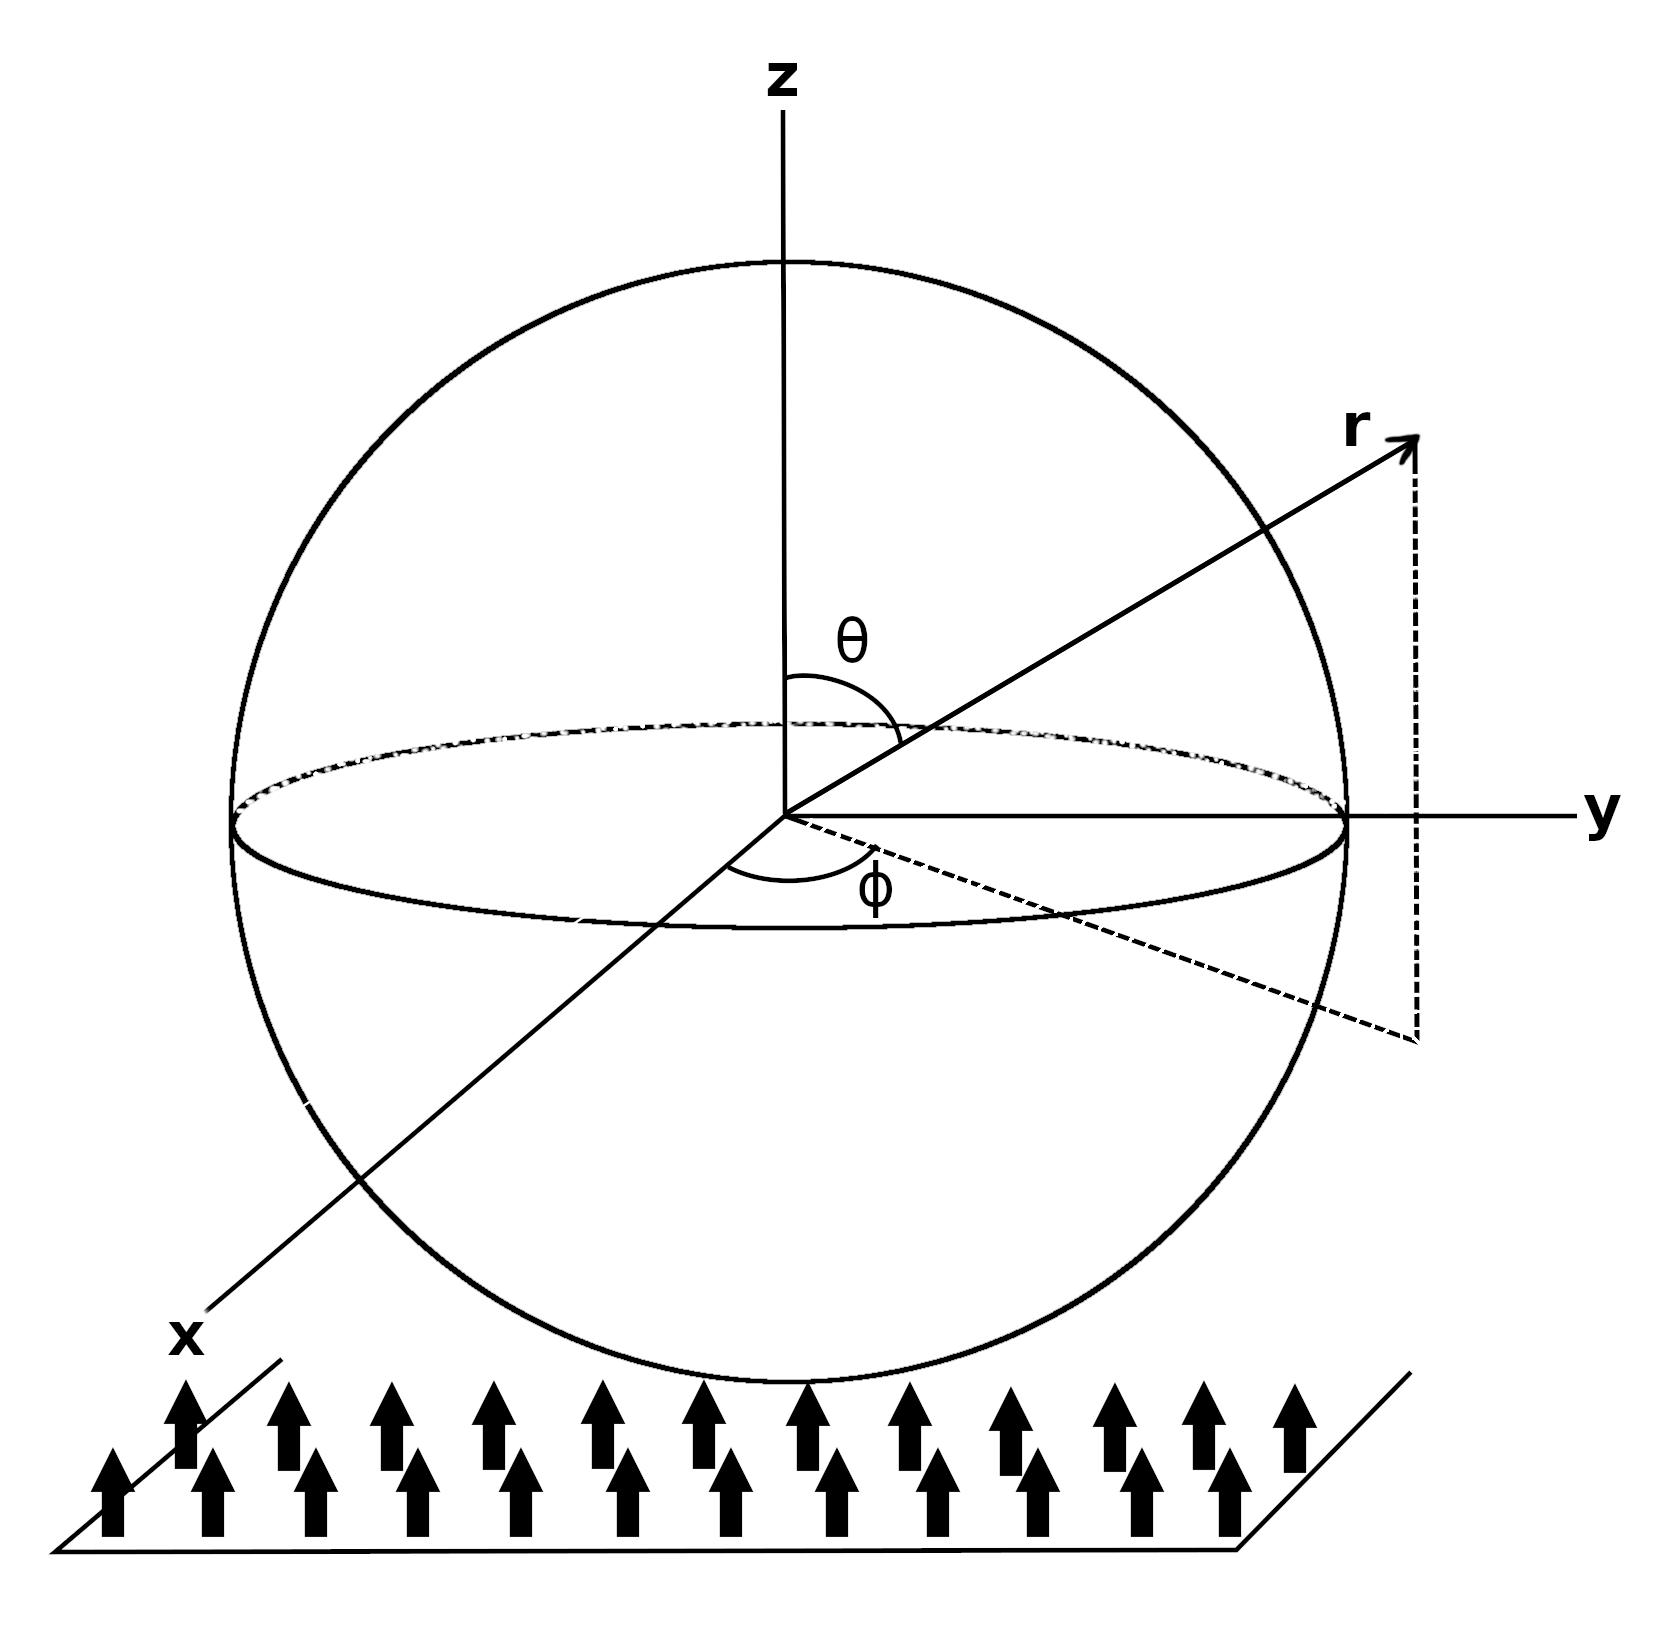
\includegraphics[width=0.4\textwidth, height=0.4\textwidth]{system.png}
    \caption{Coordinate System}
    \label{fig:system}
\end{figure}
As we can see, this reference frame is standard in most physical areas, and our incomming plane wave is going through our particle along the z-axis. That said, the aim of this project is to experimentally identify the nature of the particle resonant modes and compare with those produced by scattering calculations. Thereby, our goal is currently is to calculate this associated power, that is to say the net rate at which electromagnetic field crosses the surface A of an arbitrary sphere, which might be expressed as follow:
\begin{align}\label{eq:power_def}
W=\int_{A}^{}\textbf{S}\cdot \textbf{e}_{r}dA
\end{align}
where $\textbf{S}$ is the \textit{Pointing vector} defined as:
\begin{align}
\textbf{S} = \frac{1}{2}\Re\left\{\textbf{E}^{*} \times \textbf{H}\right\}
\end{align}
Note that an arbitrary sign can be added to (\ref{eq:power_def}) in fonction of our physical assumptions: if the Pointing vector goes out the sphere, we add a \textit{minus} sign; otherwise we let a \textit{plus} sign. In this way, we can now compute this power for the scattered electromagnetic field $(\textbf{E}_{s}, \textbf{H}_{s})$ which might be calculated thanks to (\ref{eq:an_bn}) included into the expression of the scattered field then, after a bit of mathematical manipulations, we have a literral expression for $W_{s}$. Moreover this power could be \textit{normalized}, that is to say, divided by the intensity from the incident light. Thereby, we introduce the cross section:
\begin{align}\label{eq:csca}
C_{sca}=\frac{W_{s}}{I_{i}}=\frac{2\pi}{k^{2}}\sum_{n=1}^{\infty }(2n+1)(\left| a_{n} \right|^{2}+\left| b_{n} \right|^{2})
\end{align}

In the same way, all of these previous step from (\ref{eq:w_s}) might be re-used for any other fields instead of the field $(\textbf{E}_{s}, \textbf{H}_{s})$. Until now, only the light scattered by the particle was studied thanks to three fields: $(\textbf{E}_{i}, \textbf{H}_{i})$, $(\textbf{E}_{s}, \textbf{H}_{s})$ and $(\textbf{E}_{I}, \textbf{H}_{I})$. However, it is possible to express a variable of extinction, opposed to the scattering \textit{power} $W_{s}$, due to the interaction between the electromagnetic plane wave and our particle:
\begin{align}\label{eq:wext_ws_wa}
W_{ext} = W_{s} + W_{a}
\end{align}
This additional term, combined with the \textit{total power} $W_{a}$, should be easily understood through a \textit{power balance}, that is to say an energy balance replaced by the equivalent power. Indeed, if we denote $W_{a}$ the amount of power which was varying during the interaction ($W_{a} > 0$ means that power is absorbed within the particle), it might be possible to write the following:
\begin{align}
W_{a} = W_{i} - W_{s} + W_{ext}
\end{align}
As our actual medium is nonabsorbing, the \textit{incident power} $W_{i}$ vanishes identically and we retrieve the relation (\ref{eq:wext_ws_wa}). Now, the extinction \textit{power} might be evaluated in fonction of our previous vector spherical harmonic terms:
\begin{equation}
\begin{aligned}
W_{ext}=\frac{1}{2}\int_{\phi=0}^{2\pi}\int_{\theta=0}^{\pi} (&\Re\{E_{i\phi}H^{*}_{s\theta} - E_{i\theta}H^{*}_{s\phi}\}\; +\\
&\Re\{E_{s\phi}H^{*}_{i\theta} - E_{s\theta}H^{*}_{i\phi}\}) \\
&r^{2}\sin\theta d\theta d\phi
\end{aligned}
\end{equation}
and, as stated above in (\ref{eq:csca}), we finally obtain the extinction cross section when dividing by the indicident light intensity:
\begin{align}\label{eq:cext}
C_{ext}=\frac{W_{ext}}{I_{i}}=\frac{2\pi}{k^{2}}\sum_{n=1}^{\infty }(2n+1)Re\left\{a_{n} + b_{n} \right\}
\end{align}

At last, we have calculated and theoretically established the expression of two general terms which are closely related to the spectrum we measure experimentally: $C_{sca}$ and $C_{ext}$. It is important to note that these cross section are, not only dependent on, but also strongly linked to our starting assumptions, that is to say our input variables like the radius $a$ or the refractive index $N$. Thereby, $C_{sca}$ and $C_{ext}$ are directly reliant on the size of our studied particle.

\section{Simulations}

\subsection{Equations Adjustment}

First at all, our main issue to numerically compute the cross sections $C_{sca}$ and $C_{ext}$ is to calculate the associated scattering coefficients $a_{n}$ and $b_{n}$. Globally, these two numbers are obtained through Bessel functions as we can see from (\ref{eq:an_bn}) and our goal is to retrieve each value of them between a certain range of wavelength in order to obtain a kind of spectrum. However, due to the size of our nanoparticle close to the incident wavelength included in a visible range, the variable $\rho=kr$, as a dependency for the Bessel functions, is also restrained into a small range of value close to zero along the x-axis. In fact, in the context of a computer, these targeted values could be too sensitive to be calculated with a reasonably high precision. Thereby, we could introduce the \textit{logarithmic derivative}:
\begin{align}
D_{n}(\rho)=\frac{d}{d\rho}\ln[\psi_{n}(\rho)]
\end{align}
Thanks to this additional definition, we are expanding the range of hit values and decreasing the sensitivity. In this way, we can rearrange the expressions of $a_{n}$ and $b_{n}$ from (\ref{eq:an_bn}):
\begin{equation}
\begin{aligned}
a_{n}&=\frac{[D_{n}(mx)/m + n/x]\psi_{n}(x)-\psi_{n-1}(x)}{[D_{n}(mx)/m + n/x]\xi_{n}(x)-\xi_{n-1}(x)}\\
b_{n}&=\frac{[mD_{n}(mx) + n/x]\psi_{n}(x)-\psi_{n-1}(x)}{[mD_{n}(mx) + n/x]\xi_{n}(x)-\xi_{n-1}(x)}
\end{aligned}
\end{equation}
where we have used the recurrence relation:
\begin{align}
z^{'}_{n}(x)=z_{n-1}(x)-\frac{nz_{n}(x)}{x}
\end{align}
with $z_{n}$ replaced by $\psi_{n}$ or $\xi_{n}$. Note that $x$ is not a constant because of its dependency through $\lambda$ that we are going to slide along our targeted range. Moreover, due to the recurrence relations of Bessel functions explained below, in the next subsection, $D_{n}$ also satisfies the following relation:
\begin{align}\label{eq:rec_dn}
D_{n-1}(\rho)=\frac{n}{\rho}-\frac{1}{D_{n}(\rho)+n/\rho}
\end{align}
Because of the link existing between $D_{n}$ and Bessel functions, this previous recurrence (\ref{eq:rec_dn}) should be runned downwardly, that is to say begining with the higher $n$ owned by the scattering coefficients, in order to avoid the unstability of our computation as stated in the subsection below. Otherwise, the calculated data could be rapidly \textit{flawed} while $n$ is increasing.

\subsection{Computation of Bessel Functions}

Then, our last issue is to numerically compute the spherical Bessel functions, as the first, second and the associated Hankel functions or even the Ricatti-Bessel functions. Hopefully, in our preferred scientific language that is \textit{Python}, all of these features are already implemented. Thereby, as a first approach and taking into account that \textit{Mie Theory} is not really heavy, it is completly useless and counterproductive to re-write this mathematic area. However, it could be interesting to speed up the computation thanks to a low-level programming language, or more generally, a compiled one. At least, for a better understanding of the computation, we can define a way to numerically implement these tools.

To contextually replace our problem, these Bessel functions are introduced in our theory through the resolution of the radial part (\ref{eq:radial_part}) in order to get a global expression of the generating couple of function $\psi_{emn}$ and $\psi_{omn}$. Involving spherical coordinates in our calculation, we must use the spherical Bessel functions $j_{n}$ and $y_{n}$ which are a special case of general Bessel functions $J_{n}$ and $Y_{n}$ solving the Bessel's differential equation:
\begin{align}
x^{2}\frac{d^{2}y}{dx^{2}} + x\frac{dy}{dx} + (x^{2} - \alpha^{2})y = 0
\end{align}
where $\alpha$ is a complex number without restriction. Thereby, we have the following definitions:
\begin{align}
j_{n}(x)=\sqrt{\frac{\pi}{2x}}J_{n+\frac{1}{2}}(x) \qquad y_{n}(x)=\sqrt{\frac{\pi}{2x}}Y_{n+\frac{1}{2}}(x)
\end{align}
Note that the actual $x$ might be real or a complex value and is, by definition, different from all previous sections.

After some mathematics calculation, it is possible to demonstrate the following recurrence relations:
\begin{align}\label{eq:rec_sph_bess}
\frac{2n+1}{x}z_{n}(x) &= z_{n-1}(x) + z_{n+1}(x)\\
(2n+1)\frac{d}{dx}z_{n}(x) &= nz_{n-1}(x) - (n+1)z_{n+1}(x)
\end{align}
where $z_{n}$ is either $j_{n}$ or $y_{n}$. Thanks to these previous equations (\ref{eq:rec_sph_bess}), and given the two first exact expression for the spherical Bessel functions, we can theoretically obtain all wished order $n$. So, \textit{by hand}, we have the following:
\begin{equation}
\begin{aligned}
j_{0}(x)=\frac{\sin(x)}{x} \qquad &j_{1}(x)=\frac{\sin(x)}{x^{2}} - \frac{\cos(x)}{x}\\
y_{0}(x)=-\frac{\cos(x)}{x} \qquad &y_{1}(x)=-\frac{\cos(x)}{x^{2}}-\frac{\sin(x)}{x}
\end{aligned}
\end{equation}
with the associated figures:
\begin{figure}[h]
    \centering
    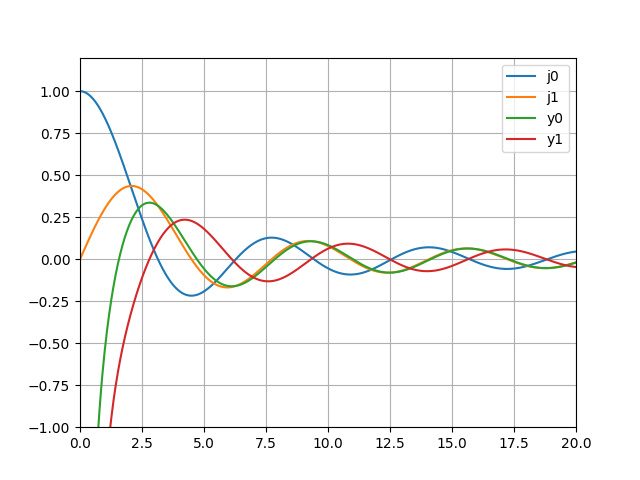
\includegraphics[width=0.5\textwidth, height=0.5\textwidth]{jnyn.png}
    \caption{$j_{0}$, $j_{1}$ with $y_{0}$, $y_{1}$}
    \label{fig:jnyn}
\end{figure}

Thereby, by inverting the main recurrence relations (\ref{eq:rec_sph_bess}) into this way:
\begin{align}\label{eq:sph_bess_up_rec}
z_{n+1}(x) &= \frac{2n+1}{x}z_{n}(x) - z_{n-1}(x)
\end{align}
we should be able to compute the next order $n=2$ for a given $x$ either real or complex. Continuing with the same idea, we can obtain $j_{3}$, $j_{4}$... coupled with the associated $y_{n}$. This way to compute all wished spherical Bessel function, or more generally any function recursively defined, from the lowest order $n=0$ reaching the highest order $n=\infty$, is commonly called an \textit{upward recurrence}. Assuming that we have in our possession a couple of spherical Bessel function at the order $n=i$ and $n=i+1$, an opposed computation from the previous one, should allow us to recursively reach $n=0$: 
\begin{align}\label{eq:sph_bess_down_rec}
z_{n-1}(x) &= \frac{2n+1}{x}z_{n}(x) - z_{n+1}(x)
\end{align}
that is called a \textit{downward recurrence} because of the decrement of $n$ for each calculated value. Despite these two recursive ways are strictly equivalent from a mathematical point of view, there is a not negligible difference between them. Indeed, taking into account boundaries of coding number (currently 64 bit for a common \textit{float}) and the behavior of spherical bessel functions, it is possible, but tough, to demonstrate either the stability or the unstability for the first and second kind calculated through downward or upward reccurency. Otherwise, by a \textit{hand} way, we can easily retrieve these theoritical results by comparing our calculations with exact curves already tabulated:
\begin{itemize}
\item Stable by \textbf{upward} recurrency: 
\begin{itemize}
\item[*]$y_{n}, \forall x$
\item[*]$j_{n}$, if $|x| \geqslant n$
\end{itemize}
\item Stable by \textbf{downward} reccurency:
\begin{itemize}
\item[*]$j_{n}$, if $|x| < n$
\end{itemize}
\end{itemize}
assuming that $\Re\{x\} \in\mathbb{R}_{+}$. Now, we can think about the programming steps in order to compute our spherical Bessel functions of the first and second kind through an upward recurrency: we get $j_{0}$/$y_{0}$ and $j_{1}$/$y_{1}$ from a given $x$ then, thanks to (\ref{eq:sph_bess_up_rec}), we compute all required order $j_{n}$/$y_{n}$ with $n \geqslant 2$. However, a question remains in a downward reccurency: How to get starting Bessel function values for higher order $n=i$ and $n=i+1$?

Theoretically, it is well know that Bessel functions of the first kind $J_{n}$ satistfies the following relation:
\begin{align}
\forall\,x\,|\,Re\{x\} \in\mathbb{R}_{+}, \lim_{n \to \infty } J_{n}(x)=0
\end{align}
Thereby a common approach, called the \textit{Miller} method, is to suppose that our targeted higher order $i$ is arbitrary equal to $1$ whereas the $i+1$ order is null. Afterward, we can easily pull down the order thanks to (\ref{eq:sph_bess_down_rec}). Once we obtain the first order $n=0$, because of the linearity of our recurrence relations, we \textit{normalize} this serie by the true value of $j_{0}(x)$. 

For example:
\begin{equation}\label{eq:j_computed}
\begin{aligned}
j^{computed}_{i+1}(x) &= 0\\
j^{computed}_{i}(x) &= 1\\
j^{computed}_{i-1}(x) &= \frac{2i+1}{x}j^{computed}_{i}(x) - j^{computed}_{i+1}\\
&...\\
j^{computed}_{0}(x) &= \alpha
\end{aligned}
\end{equation}
Now, we can \textit{normalize}:
\begin{equation}\label{eq:j_final}
\begin{aligned}
j_{0}(x) &= \frac{\sin(x)}{x} \qquad\textnormal{(by definition)}\\
j^{final}_{0}(x) &= j^{computed}_{0}(x) \times \frac{j_{0}(x)}{\alpha} = j_{0}(x)\\
j^{final}_{1}(x) &= j^{computed}_{1}(x) \times \frac{j_{0}(x)}{\alpha}\\
&...\\
j^{final}_{i}(x) &= j^{computed}_{i}(x) \times \frac{j_{0}(x)}{\alpha}\\
\end{aligned}
\end{equation}
where $j^{final}_{X}$ is the wished result. In fact, we just have \textit{normalized} our serie $j^{computed}_{X}$ by the initial factor $\frac{j_{0}(x)}{\alpha}$. It is important to notice that any serie constructed through this way always verifies the recurrence relation (\ref{eq:sph_bess_up_rec}) and each term is, by definition, a solution of the radial part (\ref{eq:radial_part}).

Unfortunately, a last issue still remain in our downward recurrency approach. Something that is not obvious at the first glance, we see that for a given $i$ and for any $x$, the serie $j^{computed}_{X}$ always has the same value for all terms in it. That is to say, only the \textit{normalization} factor introduce the value $x$ in our final serie and, finally, $j^{computed}_{X}(x)$ is not really dependent on $x$ (we can omit this parameter afterwards). In this way, due to the mathematical shape of our recurrence relation (\ref{eq:sph_bess_down_rec}), each value of a lower computed order is bigger than its previous higher order: $j^{computed}_{0} > j^{computed}_{1} > ... > j^{computed}_{i}$. So, if we target a really high order with, for instance, $i=10^{10}$, the first order will ineluctably get a really high value. Thereby, for a computer with \textit{physical} boundaries for its numbers, this previous result will give us an invalid value for an intermediate order and all order below will be saturated with the same invalid state. In this way, the \textit{normalization} step is impossible because $\alpha$ in (\ref{eq:j_final}) will own a \textit{NaN} value (that is a computer overflow indicator). Even if, for a first approximation, we use the ten first order for calculation, this phenomenon will be rapidly visible even for our range of value (from $n=50$) and it could be intersting to avoid this \textit{blocking} state. So, the first solution proposed in many other articles treating the \textit{Mie Theorie}, or more generally the computation of Bessel functions, is to set an arbitray minimal value for $i$, that is to say $10^{-10}$ instead of $1$. However, this method will only postpone the phenomenon. A second solution is to divide the downward reccurency into multiple chunks. As mentioned above, $j^{computed}_{X}$ is recursive and completly dependent on the targeted order $i$. In fact, if we want $i=1000$ as a final order, we can calculate $j^{computed}_{X}$ from $n=0$ to $n=50$ (stability limit) and apply a normalization as previously stated for this first chunk. Secondly, we compute a second chunk starting from $n=50$ to $n=100$ (actually, the computation begins with $n=100$ because of the downward behavior). Then, it is possible to assume that $\{j^{computed}_{0}...j^{computed}_{50}\} = \{j^{computed}_{50}...j^{computed}_{100}\}$ due to the arbitrary recurrence relation. For the second chunk, we can normalize it by $j^{computed}_{50}$ from the first chunk, itself normalized by the exact $j_{0}(x)$ (which is not arbitrary but dependent on $x$). This method is chain-shaped and we recursively advance, chunk by chunk to finally obtain every order wished without overflowing the computer results.

\subsection{Input Variables}

At this point of our simulation part, we have to precisely fix and set our input variables, that is to say with, roughly, this following pattern:
\begin{align}
Output = Simulation(Input)
\end{align}
where $Output$ is our wished scattering and extinction cross sections. Given the relations (\ref{eq:csca}) and (\ref{eq:cext}) coupled with the expressions of $a_{n}$ and $b_{n}$ previously established, we are able to recognize these variables. Thereby, all inputs are included into (\ref{eq:def_x_m}) with refractive indices of the medium $N_{I}$ and the particle $N$, the particle's size $a$ then the wavelength $\lambda$.

First at all, let's consider the $\lambda$ variable. The problem is the following: from our theory, we send an incident monochromatic light, that is to say $\lambda=constant$ in the visible range. However, in reality, the experimental tool produce multiple monochromatic lights in order to reach all values in the visible range and compute the associated cross sections. In fact, the wavelength $\lambda$ will vary for each computation and, by the way, is an $Input$ variable. Therefore, we have $x=x(\lambda)$ and more precisely $k=k(\lambda)$

Secondly, the particle's size $a$ represents the radius of this last one. Obviously, from the purpose of this study, it is also an $Input$ variable.

Then, the refractive index of the medium, taking into account that the environment is homogenous, this last one is a constant value. Even more, if we consider that the medium is the ambiant air, it might be possible to approximate it as the void and finally set $N_{I}=1$. Moreover, we have now the following relation $m=N$.

The last variable to describe is the refractive index $N$ of our particle. At this point, we can introduce the targeted material, that is to say, the substance used into our spherical sample: silicon. As a first approximation, we can say that silicon has a constant refractive index commonly setted around $3.5$. Thereby, for $a=100^{-9}m$ and $\lambda=[206^{-9}, 826^{-9}]$ (visible range a bit extended in the \textit{UV} range), we obtain the following cross sections:
\begin{figure}[h]
    \centering
    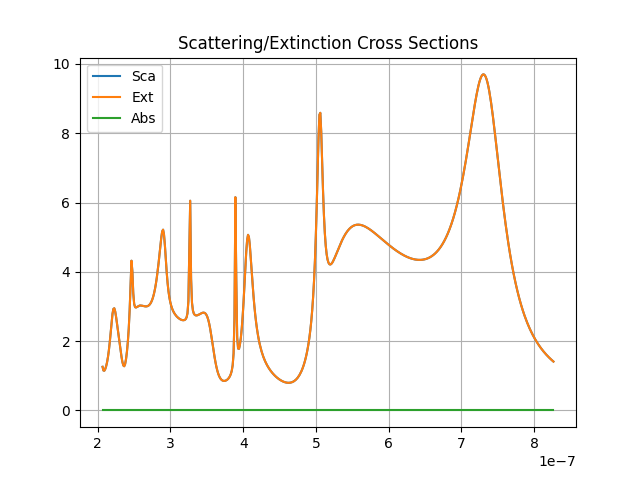
\includegraphics[width=0.5\textwidth, height=0.4\textwidth]{ri_const.png}
    \caption{Cross sections with $N=3.5$}
\end{figure}
where $Sca$ is the scattering, $Ext$ the extinction and $Abs$ the absorbtion cross section linked with (\ref{eq:wext_ws_wa}): $C_{abs} = C_{ext} - C_{sca}$. We can see that there is no absorbtion and the scattering cross section equals the extinction one. However, to properly describe physical states of matter, we have to consider that the refractive index is varying depending on the wavelength of the incident light, that is to say, $N=N(\lambda)$. In this way we obtain:
\begin{figure}[h]
    \centering
    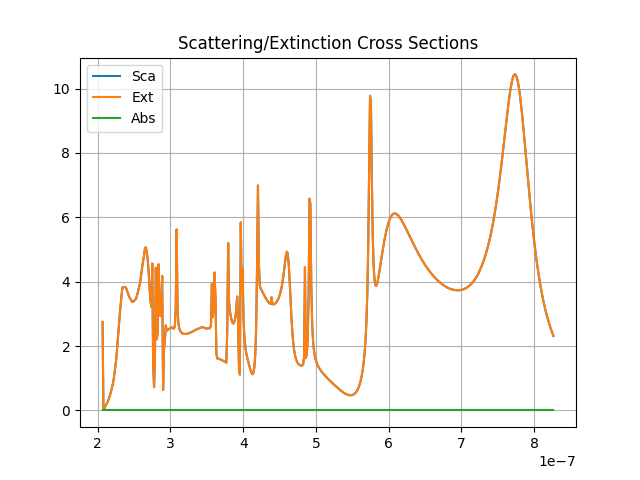
\includegraphics[width=0.5\textwidth, height=0.4\textwidth]{ri_var_real.png}
    \caption{Cross sections with $N=N(\lambda)$}
\end{figure}
where we use the real part of pre-computed refractive indices from another scientific experiment (Aspnes and Studna, 1983). We easily see that the main maximums, called \textit{Mie resonances}, are shifted to the right but this approach globally keep the previous shape. It is always remarkable that $C_{sca}=C_{ext}$. That is due to the real expression of the refractive index. Indeed, the absorbtion behavior of our material is mathematicaly implemented through the imaginary part of $N$. In this way, we should have $N=N_{re}+iN_{im}$ Thereby, when we use a complex varying index, we obtain:
\begin{figure}[h]
    \centering
    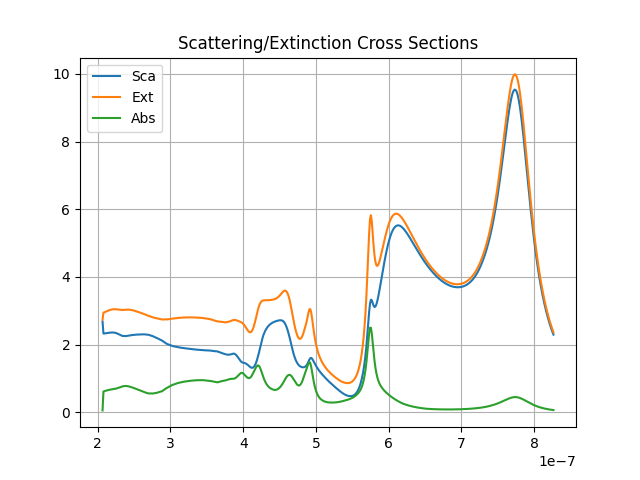
\includegraphics[width=0.5\textwidth, height=0.4\textwidth]{ri_var_complex.png}
    \caption{Cross sections with $N=N(\lambda)$ complex}
\end{figure}
Now, in addition to the previous shape then according to each Mie's resonance pike, we have a maximum of absorbtion describing the capacity of our particle to redistribute the energy of the incident light into another form, like a thermal energy. It is important to notice that the varying imaginary part doesn't change the position of the pikes in contrary to the varying real part.

Finally, our $Input$ variables are the following: $a$ (particle's size), $\lambda$ (incident light's wavelength) and $N(\lambda)$ (refractive index depending on $\lambda$).

\subsection{Results}

Finally, we are able to compute our required $Output$ which are the scattering $C_{sca}$ and extinction $C_{ext}$ cross sections. As a reminder and as stated in the end of the \textit{theory} part, these last are relevant in the study of nanoparticles because cross sections are directly linked to the size of the particle.

First at all, it could be interesting to visualize the different contributions of each terms in cross section expressions (\ref{eq:csca}) and (\ref{eq:cext}). Indeed, these two relations are primarly composed of an infinite sum which might be \textit{separated} in order to compute the associated $a_{n}$ and $b_{n}$ terms roughly as following:
\begin{align}
\sum_{n=1}^{\infty } f_{n}(a_{n}) + f_{n}(b_{n}) = \sum_{n=1}^{\infty } f_{n}(a_{n}) + \sum_{n=1}^{\infty } f_{n}(b_{n})
\end{align}
where $f_{n}(X) = \frac{2\pi}{k^{2}}(2n+1)\Re\{X\}$ in the case of $C_{ext}$ (with a similar expression for $C_{sca}$). In this way, for an arbitray particle defined by a radius of $100e^{-9}$ meters, we obtain (\ref{fig:sca_coeff}) then (\ref{fig:ext_coeff}) for the scattering and extinction cross section respectively.
\begin{figure}[h]
    \centering
    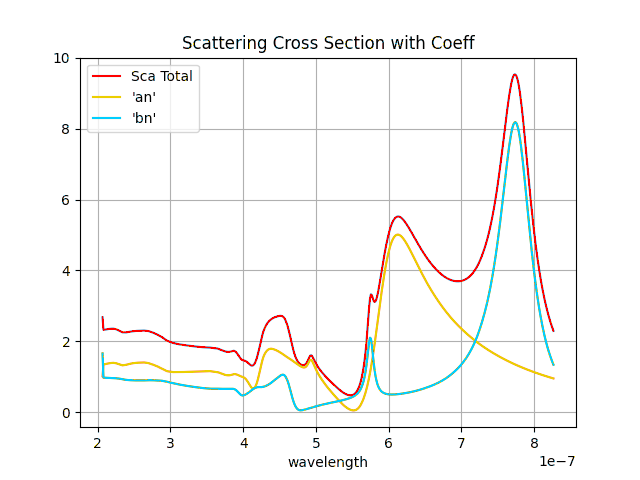
\includegraphics[width=0.5\textwidth, height=0.4\textwidth]{sca_coeff.png}
    \caption{$C_{sca}$ coefficient contributions}
    \label{fig:sca_coeff}
\end{figure}
\begin{figure}[h]
    \centering
    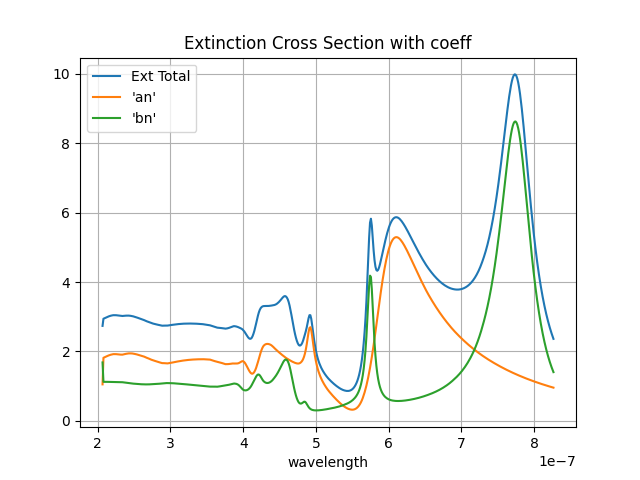
\includegraphics[width=0.5\textwidth, height=0.4\textwidth]{ext_coeff.png}
    \caption{$C_{ext}$ coefficient contributions}
    \label{fig:ext_coeff}
\end{figure}
These figures show that each local maximum is due to a heavy weighting from one or the other of the coefficients. More particularly, the global maximum called \textit{principal Mie's resonance} seems to be be generated by the second coefficient $b_{n}$ whereas the first one, $a_{n}$ influences the second global maximum which is located on the left of the first maximum.

Secondly, as stated in the previous subsection, we have three $Input$ variables that we can potentially change. Note that the incident light's wavelength is fixed by the targeted range of value for the \textit{extended}-visible light and the refractive index of our particle, depending on $\lambda$, is, him too, fixed by the material studied: silicon. Thereby, our last \textit{free} parameter is the size or more precisely the radius. Therefore, when varying this $Input$ variable, we obtain (\ref{fig:sca_var}) and (\ref{fig:ext_var}) associated to $C_{sca}$ and $C_{ext}$ for three different sizes surrounding all possible particles encountered during the experiments.
\begin{figure}[h]
    \centering
    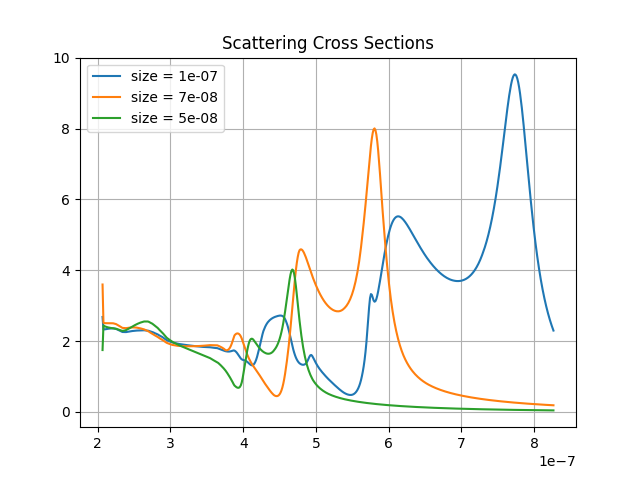
\includegraphics[width=0.5\textwidth, height=0.4\textwidth]{sca_var.png}
    \caption{$C_{sca}$ for three different sizes}
    \label{fig:sca_var}
\end{figure}
\begin{figure}[h]
    \centering
    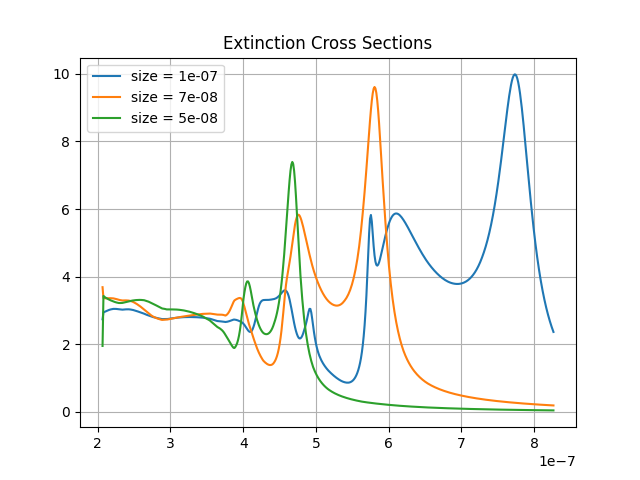
\includegraphics[width=0.5\textwidth, height=0.4\textwidth]{ext_var.png}
    \caption{$C_{ext}$ for three different sizes}
    \label{fig:ext_var}
\end{figure}
As we can see, it is possible to consider a \textit{recursive} shape which is composed by the boundary of the first and second global maximum. In fact, the principal Mie's resonance is moving left when the size decreases and reciprocally. Moreover the scale and the maximum y-value are also decreasing. However, it might be roughly possible to assess that, for our targeted range of values, this shape thus defined is moving left for smaller sizes then right for larger sizes.

After all, if we reproduce our computations with, this time, the radius as a \textit{real} free parameter instead of an arbitrary fixed value, we obtain the following figures (\ref{fig:surface_sca}) and (\ref{fig:surface_ext}) for the scattering and extinction cross sections respectively. In this way, we can easily visualize our wished $Output$ results and compare later with the collected experimental data.
\begin{figure}[h]
    \centering
    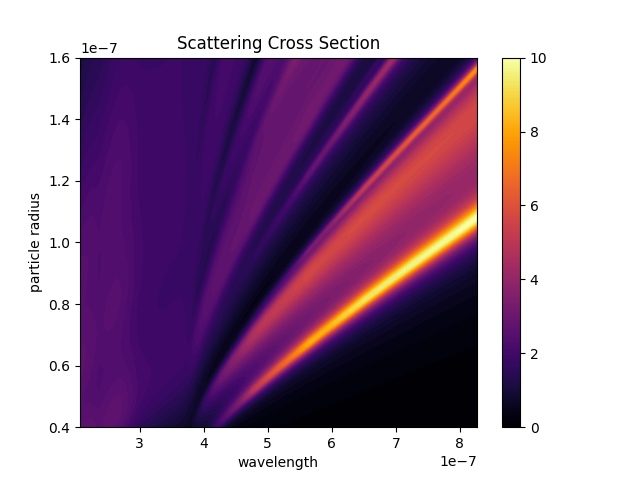
\includegraphics[width=0.5\textwidth, height=0.4\textwidth]{surface_sca.png}
    \caption{$C_{sca}$ depending on radius and wavelength}
    \label{fig:surface_sca}
\end{figure}
\begin{figure}[h]
    \centering
    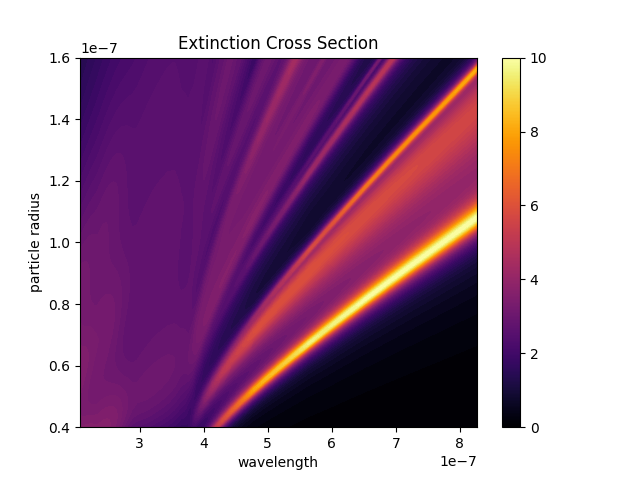
\includegraphics[width=0.5\textwidth, height=0.4\textwidth]{surface_ext.png}
    \caption{$C_{ext}$ depending on radius and wavelength}
    \label{fig:surface_ext}
\end{figure}
Now, it is obvious that, as a really first approximation in our range of values, each maximum and, more particularly, the two global maximum represented by the most intense yellow lines, could be calculated through a linear equation with a different coefficient each explaining, by the way, the compression of the defined shape for smaller radius. \textbf{Retrieve the linear equation for the principal Mie's resonance and compare}

\section{Experiments}

\subsection{Base Description}

First, let's describe the procedure to experimentally test and compare our simulation part. In theory, our studied particle should have a spherical shape and, as stated in the previous section, the associated material should be \textit{silicon}. Thereby, we are supposed to create a sample composed of spherical nanoparticles of silicon with different sizes included between $100nm$ and $200nm$ of diameter. Moreover, in order to approve our theorical approach and all of the approximation employed until now, we have to retrieve experimentally the \textit{defined shape} made up of the first and second principal Mie resonancies linked with an equivalent gradient. In fact, our different sized nanoparticles being randomly scattered on the sample, we have to collect the size of some nanoparticles coupled with both scattering and extinction cross section spectrums. In this way, we will be able to link $C_{sca}$ and $C_{ext}$ shapes according to the respective sizes to finally check if those actually fit the simulation. Therefore, the tools used to collect each spectrums associated with the size are the \textit{optical} and \textit{atomic force} microscopes respectively.

\subsection{Sample Preparation}

Chronologically, the first experimental stuff we have to realize is the preparation of the silicon nanoparticle sample.

First of all, we have to find a proper support for our different particles. In this way, we use a glass substrat which is composed of a matrix where micrometric number elements are engraved on the bottom side, in order to see and locate the position of our experiment area on this sample during observation through optical or AFM microscopes. The substrat has the particularity to be transparent which allow the light to cross it and let numbers to be visible as shown on figure (\ref{fig:substrat}).
\begin{figure}[h]
    \centering
    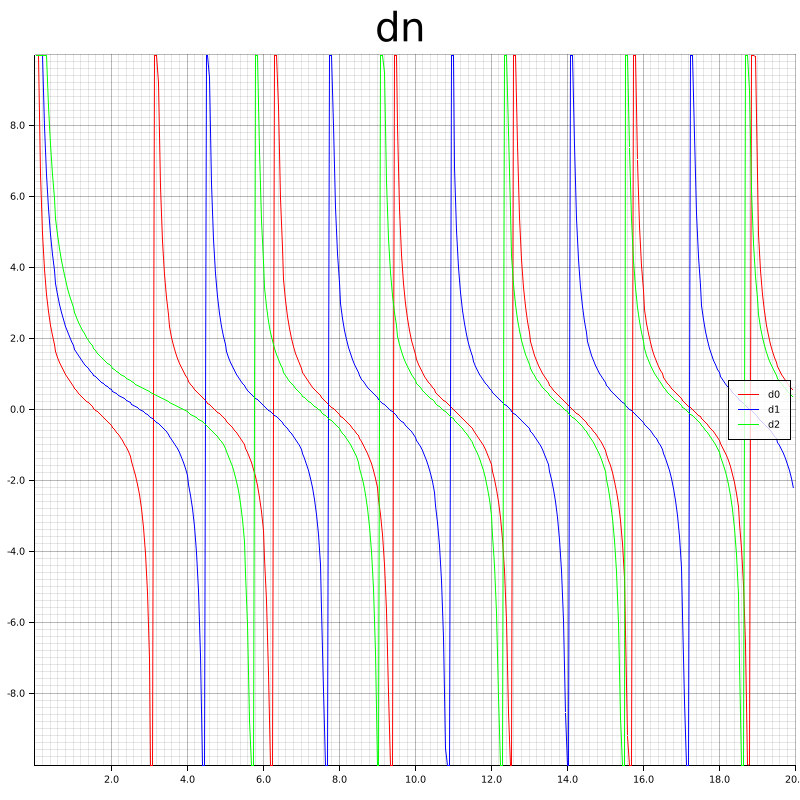
\includegraphics[width=0.4\textwidth, height=0.35\textwidth]{dn.png}
    \caption{glass substrat}
    \label{fig:substrat}
\end{figure}
Moreover, our goal being to put nanoparticles on this substrat, we have the following layers described on figure (\ref{fig:substrat_layers}).
\begin{figure}[h]
    \centering
    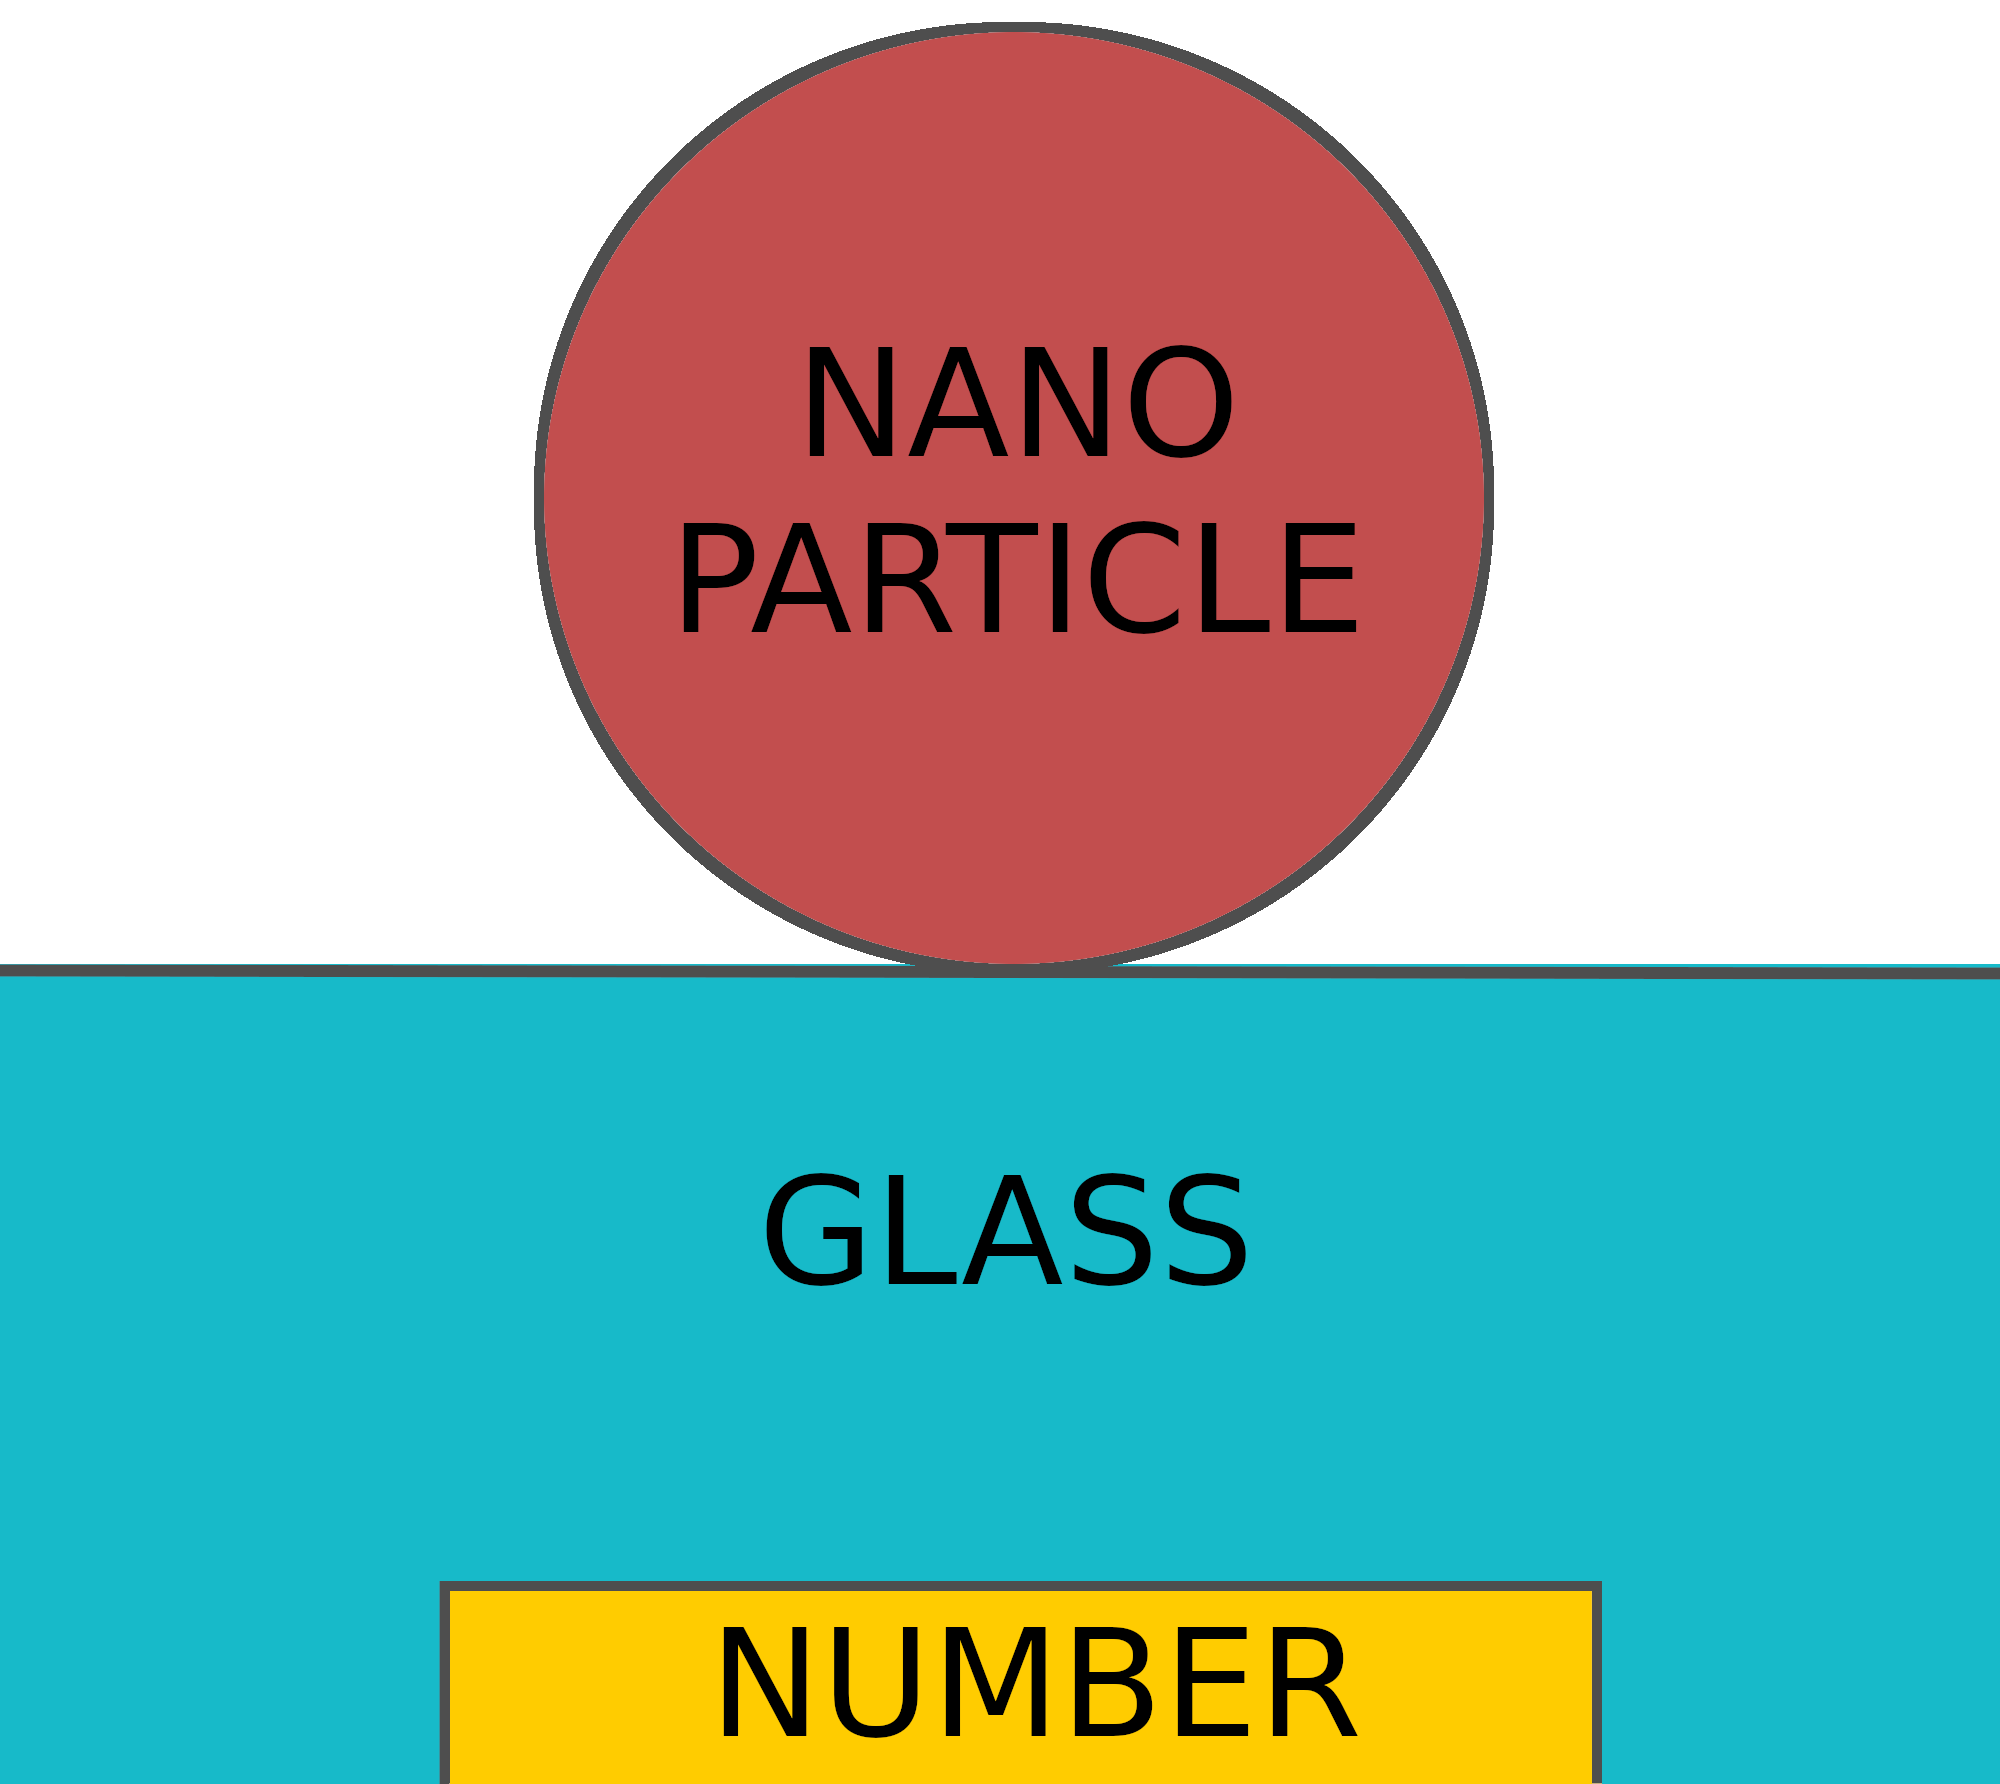
\includegraphics[width=0.4\textwidth, height=0.35\textwidth]{substrat_layers.png}
    \caption{Substrat Layers (Not To Scale)}
    \label{fig:substrat_layers}
\end{figure}
From a technical point of view, the base glass substrat is too large to be placed on the different microscope. Thereby, this last one must be broke into several pieces, each with dimensions smaller than $2 \times 2 cm$.

Secondly, we have to physically produce silicon nanoparticles with \textit{random} sizes included between $50 nm$ and $100 nm$ in radius. Hopefully, this step is realized thanks to another research team from the \textit{DTU} (see ...). Globally, they are created from $SiO$ lumps annealed at, approximately, $1500 \degree C$ then etched to produce $Si$ nanoparticles in a solution.

Finally, these nanoparticles are placed on the glass substrat pieces thanks to a micropipette: we put a droplet of around $10$ microliter on each chip. Afterward, we must either dry in air, or blow dry to progressively remove water from the samples. In the end, our silicon nanoparticles are \textit{dropcasted}.

\subsection{Optical Microscope}

Now, our goal is to collect the spectrum from some intersting particles, preferably with a large distribution of size starting from $50 nm$ to $100 nm$ in radius. In order to select these wished particle and get the equivalent of scattering cross and extinction cross section, we have to use the \textit{optical} microscope. Globally, this tool is working like a \textit{basic} microscope, numerically connected to a computer where where recorded images might be seen through a normal screen, composed of $3$ different scopes ($\times 10$, ask Kirstine) and working with $2$ different modes of lighting: \textit{bright} and \textit{dark} field. The first one mode is a standard lighting: the ingoing light is emitted from the top of the device and the reflecting light is also collected from the top to be transfered to a detector and finally to the computer or directly to the \textit{user-eyes}.
\begin{figure}[h]
    \centering
    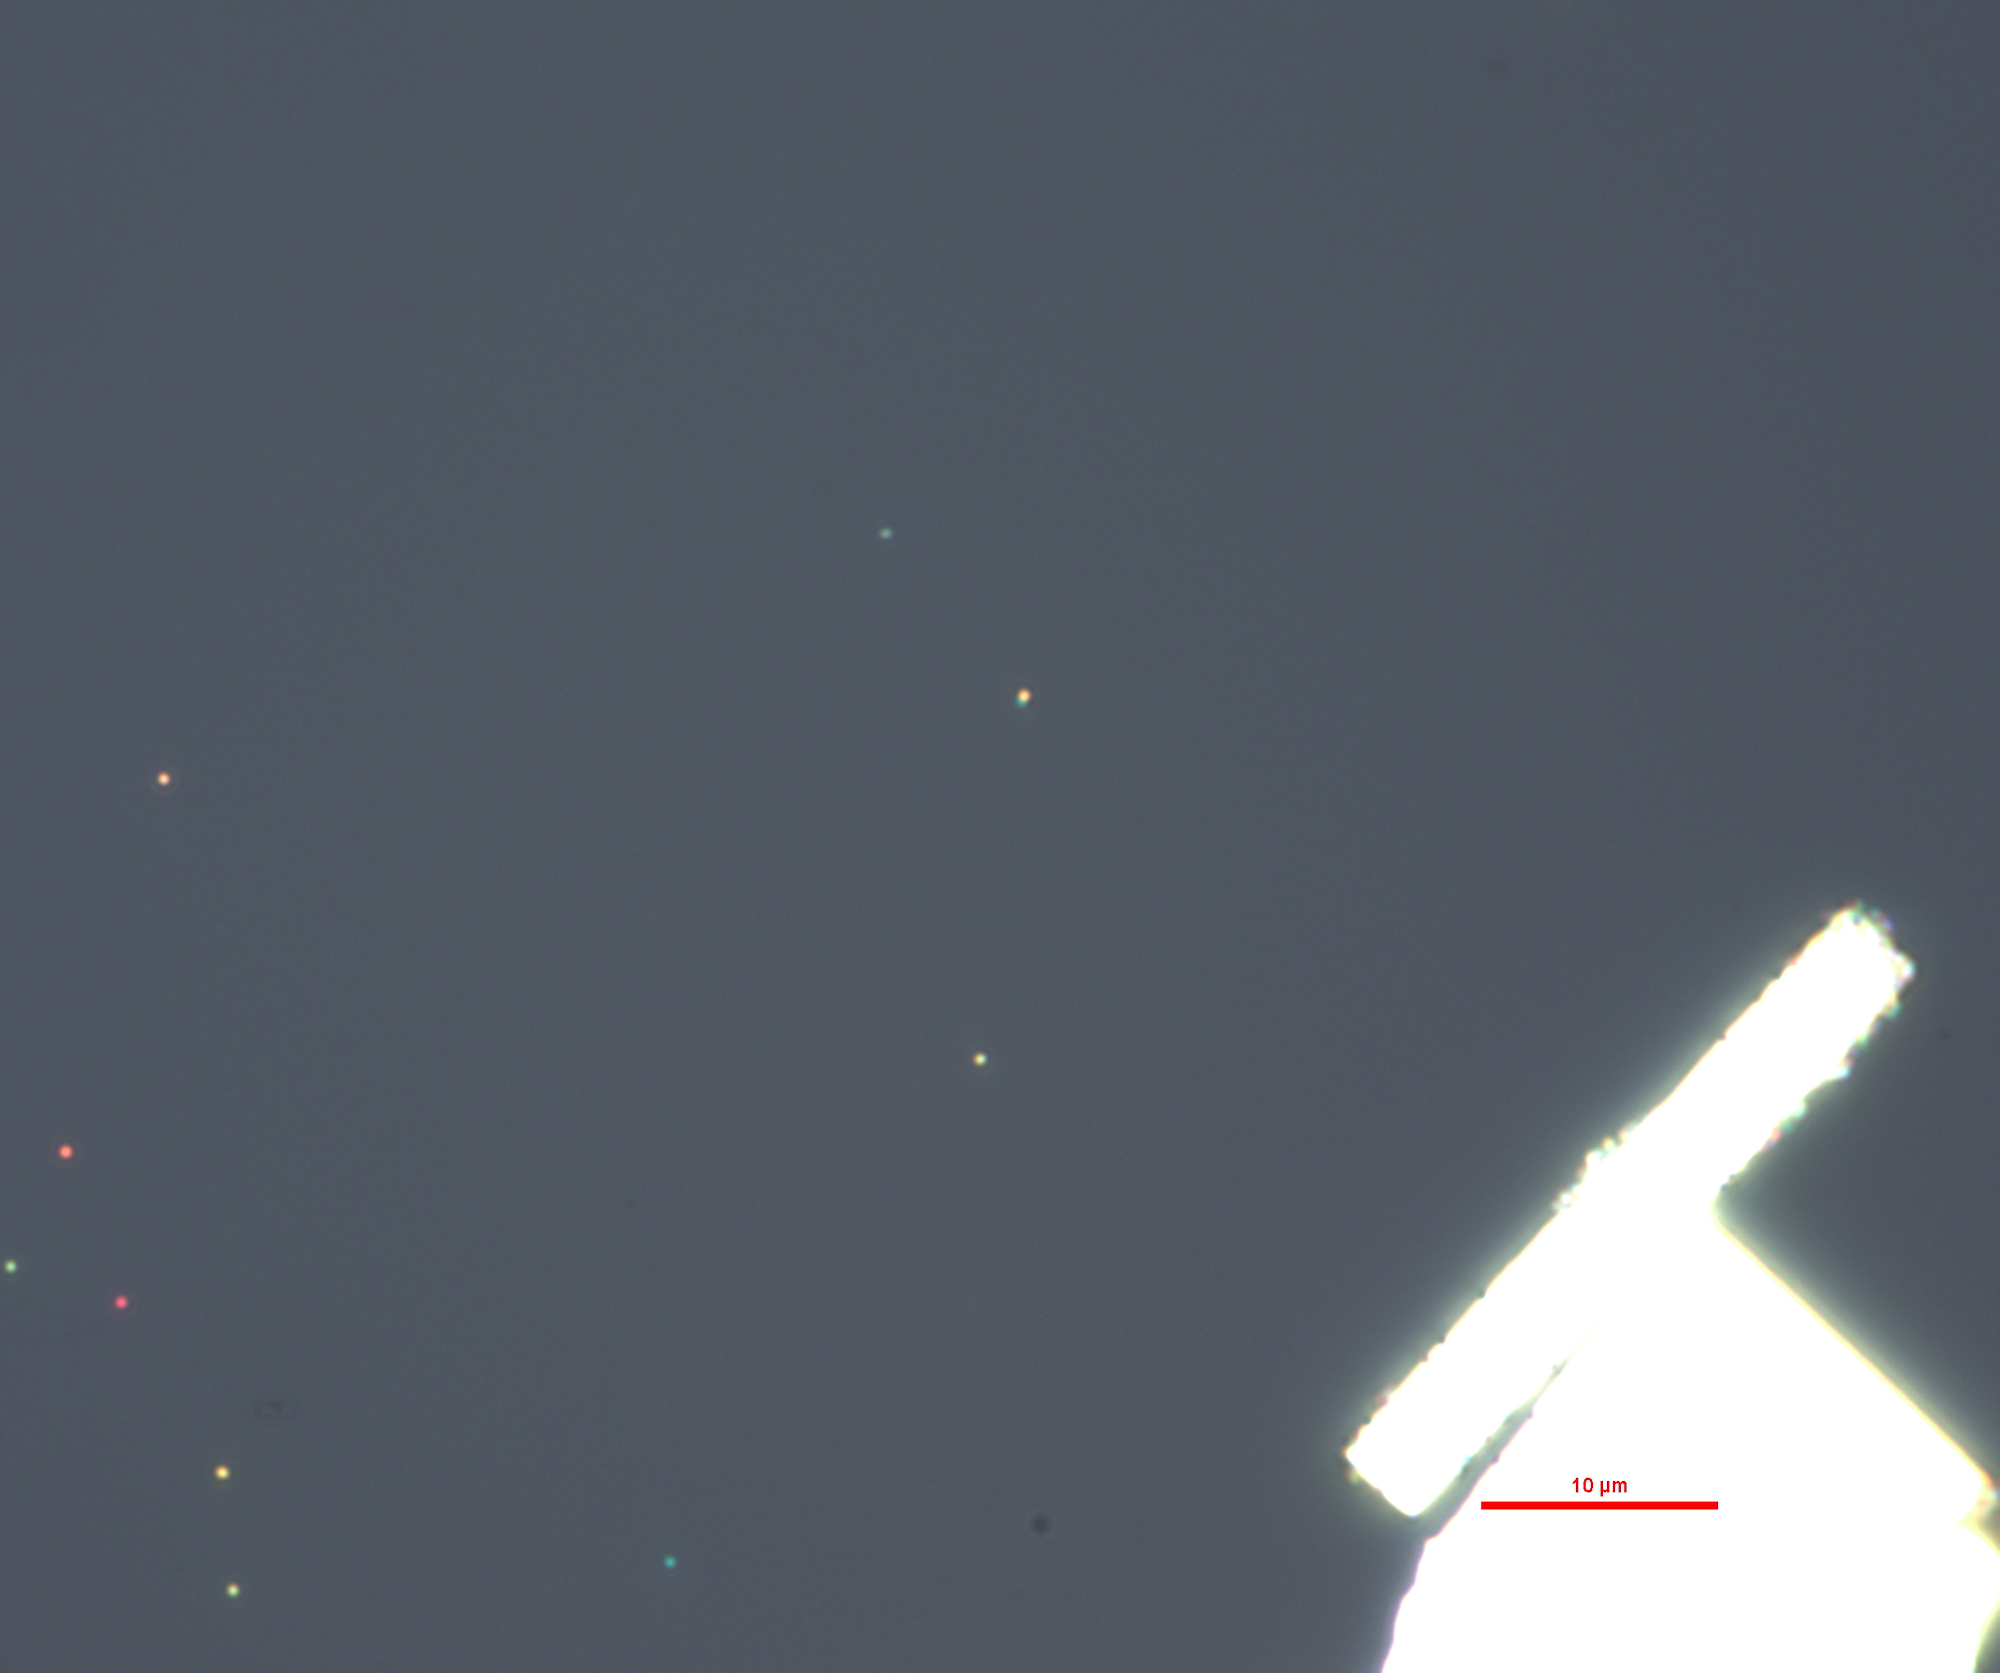
\includegraphics[width=0.4\textwidth, height=0.35\textwidth]{bright_field_ex.png}
    \caption{Bright Field Example}
    \label{fig:bright_field_ex}
\end{figure}
Secondly, the \textit{dark field} is used to increase the contrast and avoid the emitted light to be directly collected. Indeed in our case, with the standard mode, all silicon nanoparticles look generally the same, that is to say, the reflected light is pretty close due to the slight difference between each sphere (we are talking about less than $50 nm$ in radius). Thereby, the \textit{dark field} mode allow us to send an incident light and only catch the scattered light as shown on figure (\ref{fig:dark_field_working}). Unfortunately, it means that only the scattering cross section should be reached for comparison with simulation results.
\begin{figure}[h]
    \centering
    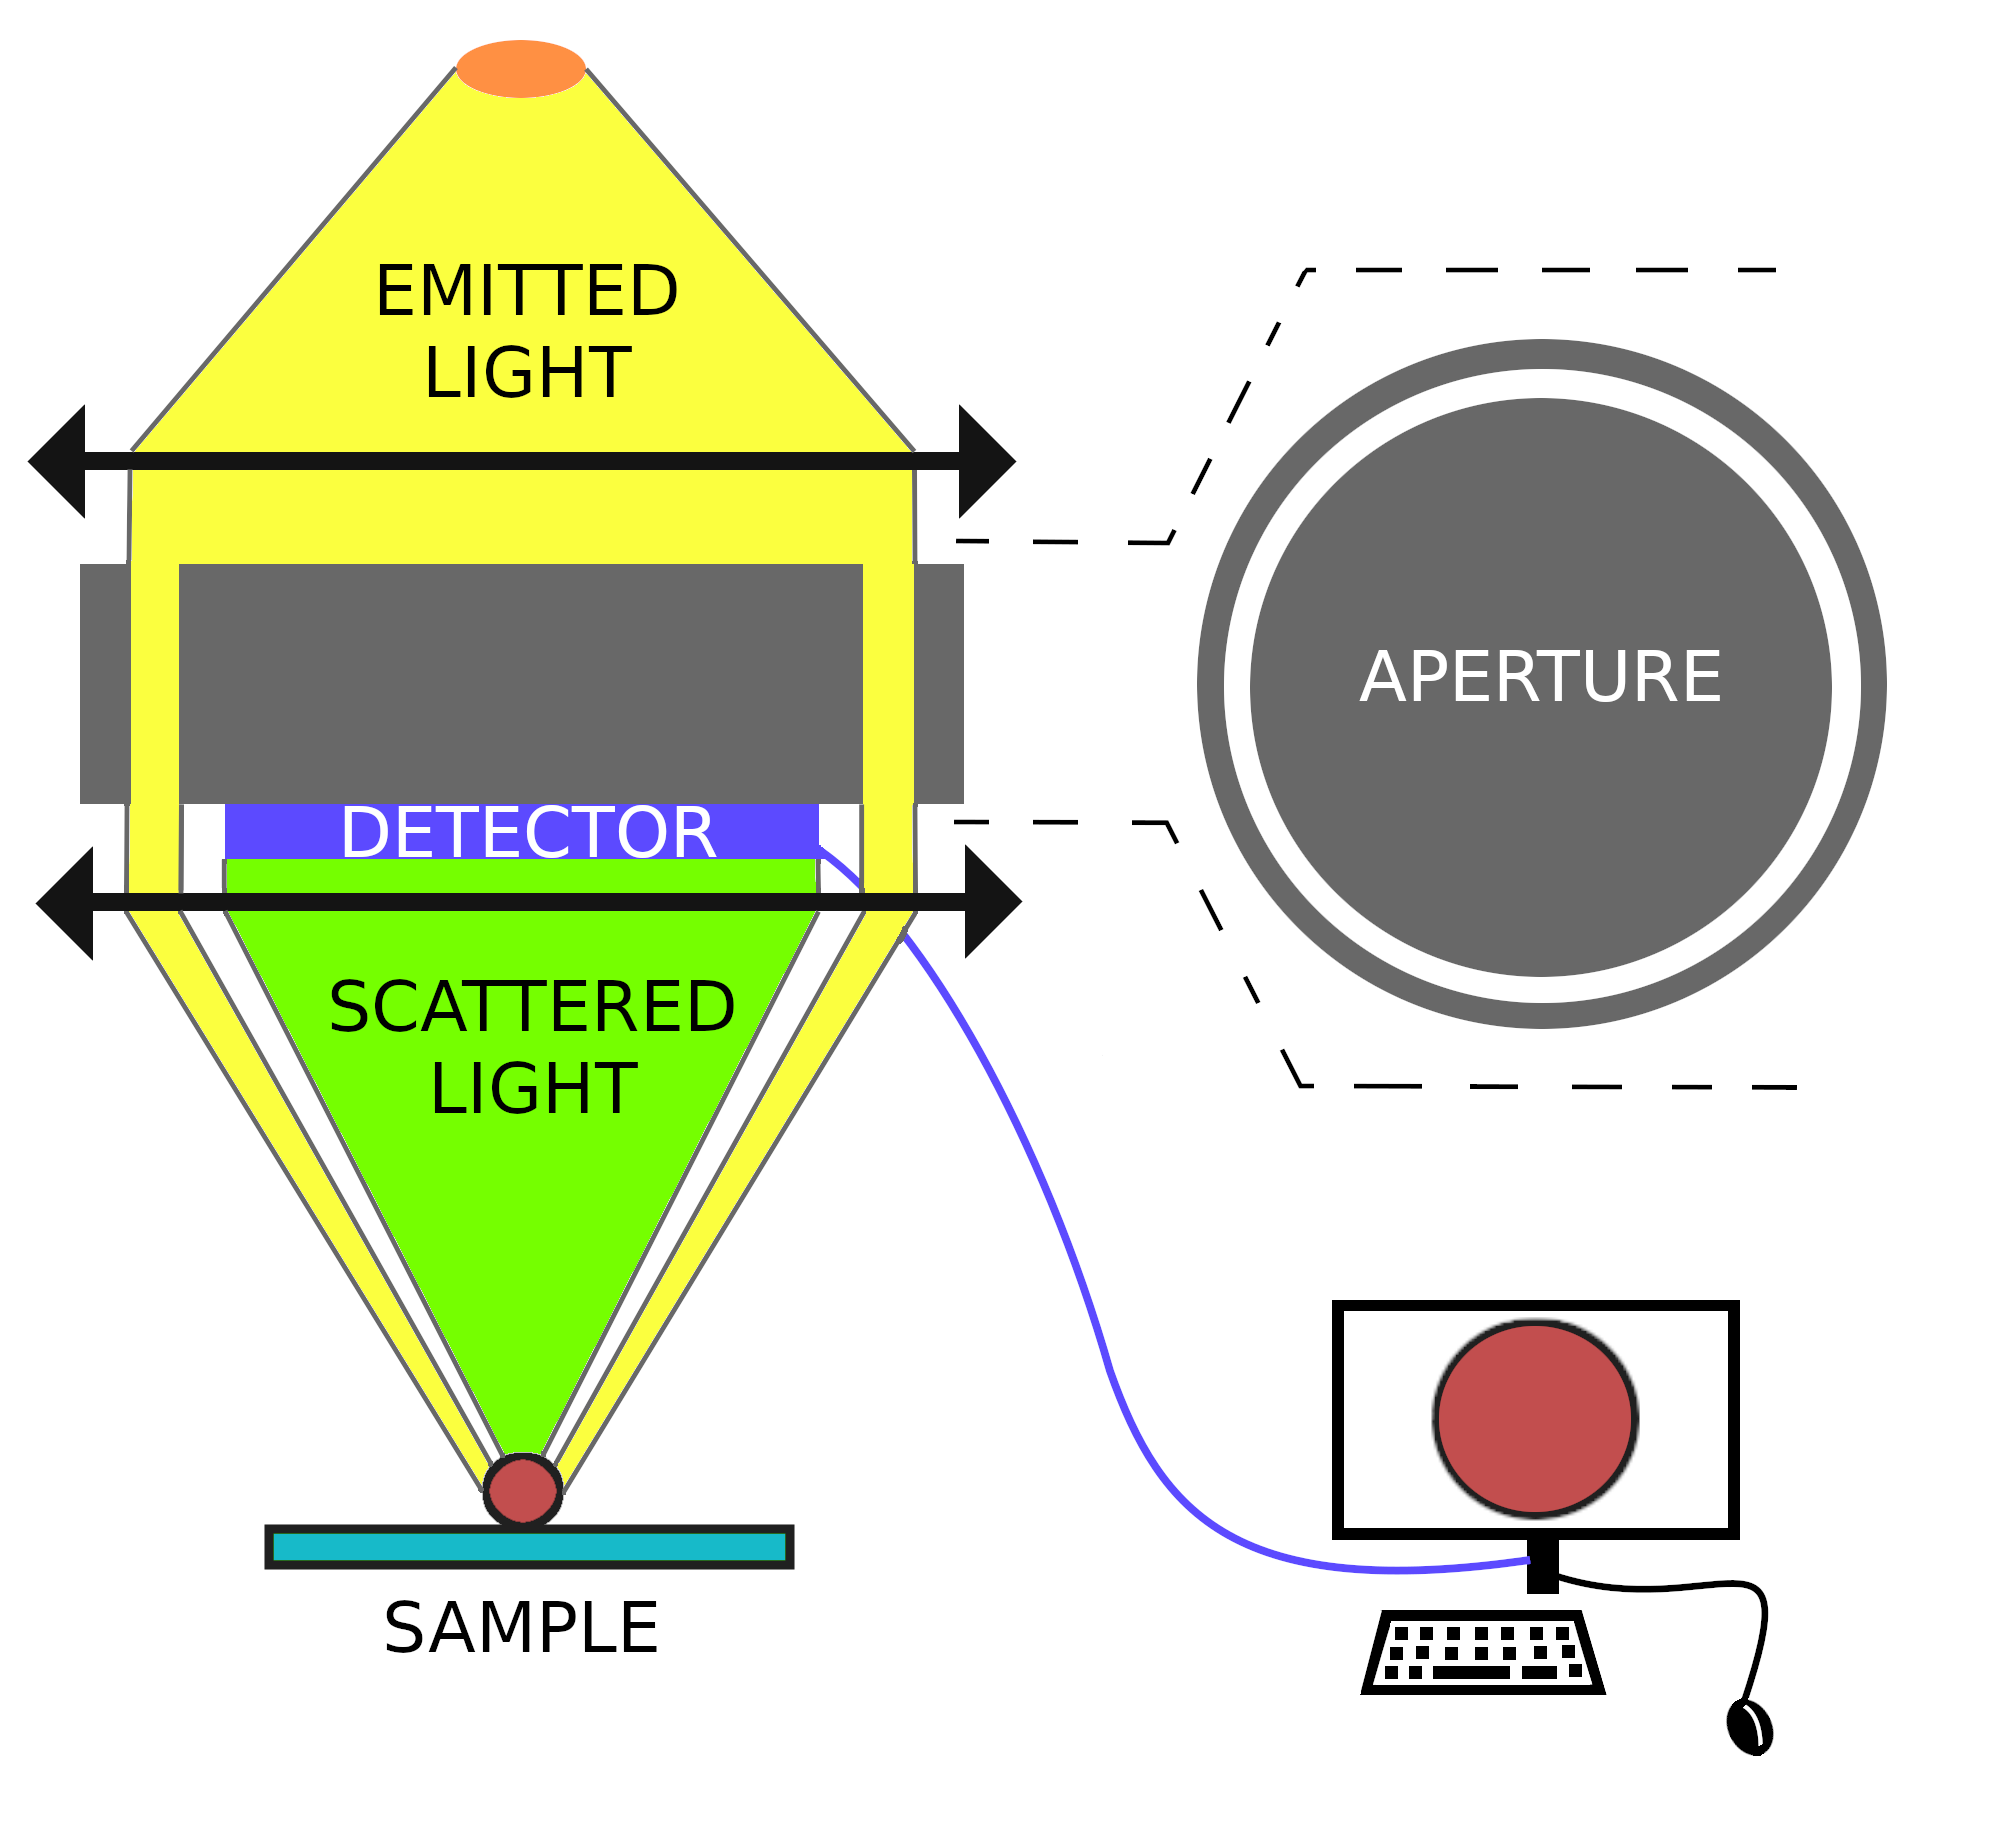
\includegraphics[width=0.4\textwidth, height=0.37\textwidth]{dark_field_working.png}
    \caption{Dark Field Working}
    \label{fig:dark_field_working}
\end{figure}
As we can see, the incident direction is described as the edge of a cone and, due to the refractive index of the studied sample (not only nanospheres), the scattered light is collected inside the same cone.
\begin{figure}[h]
    \centering
    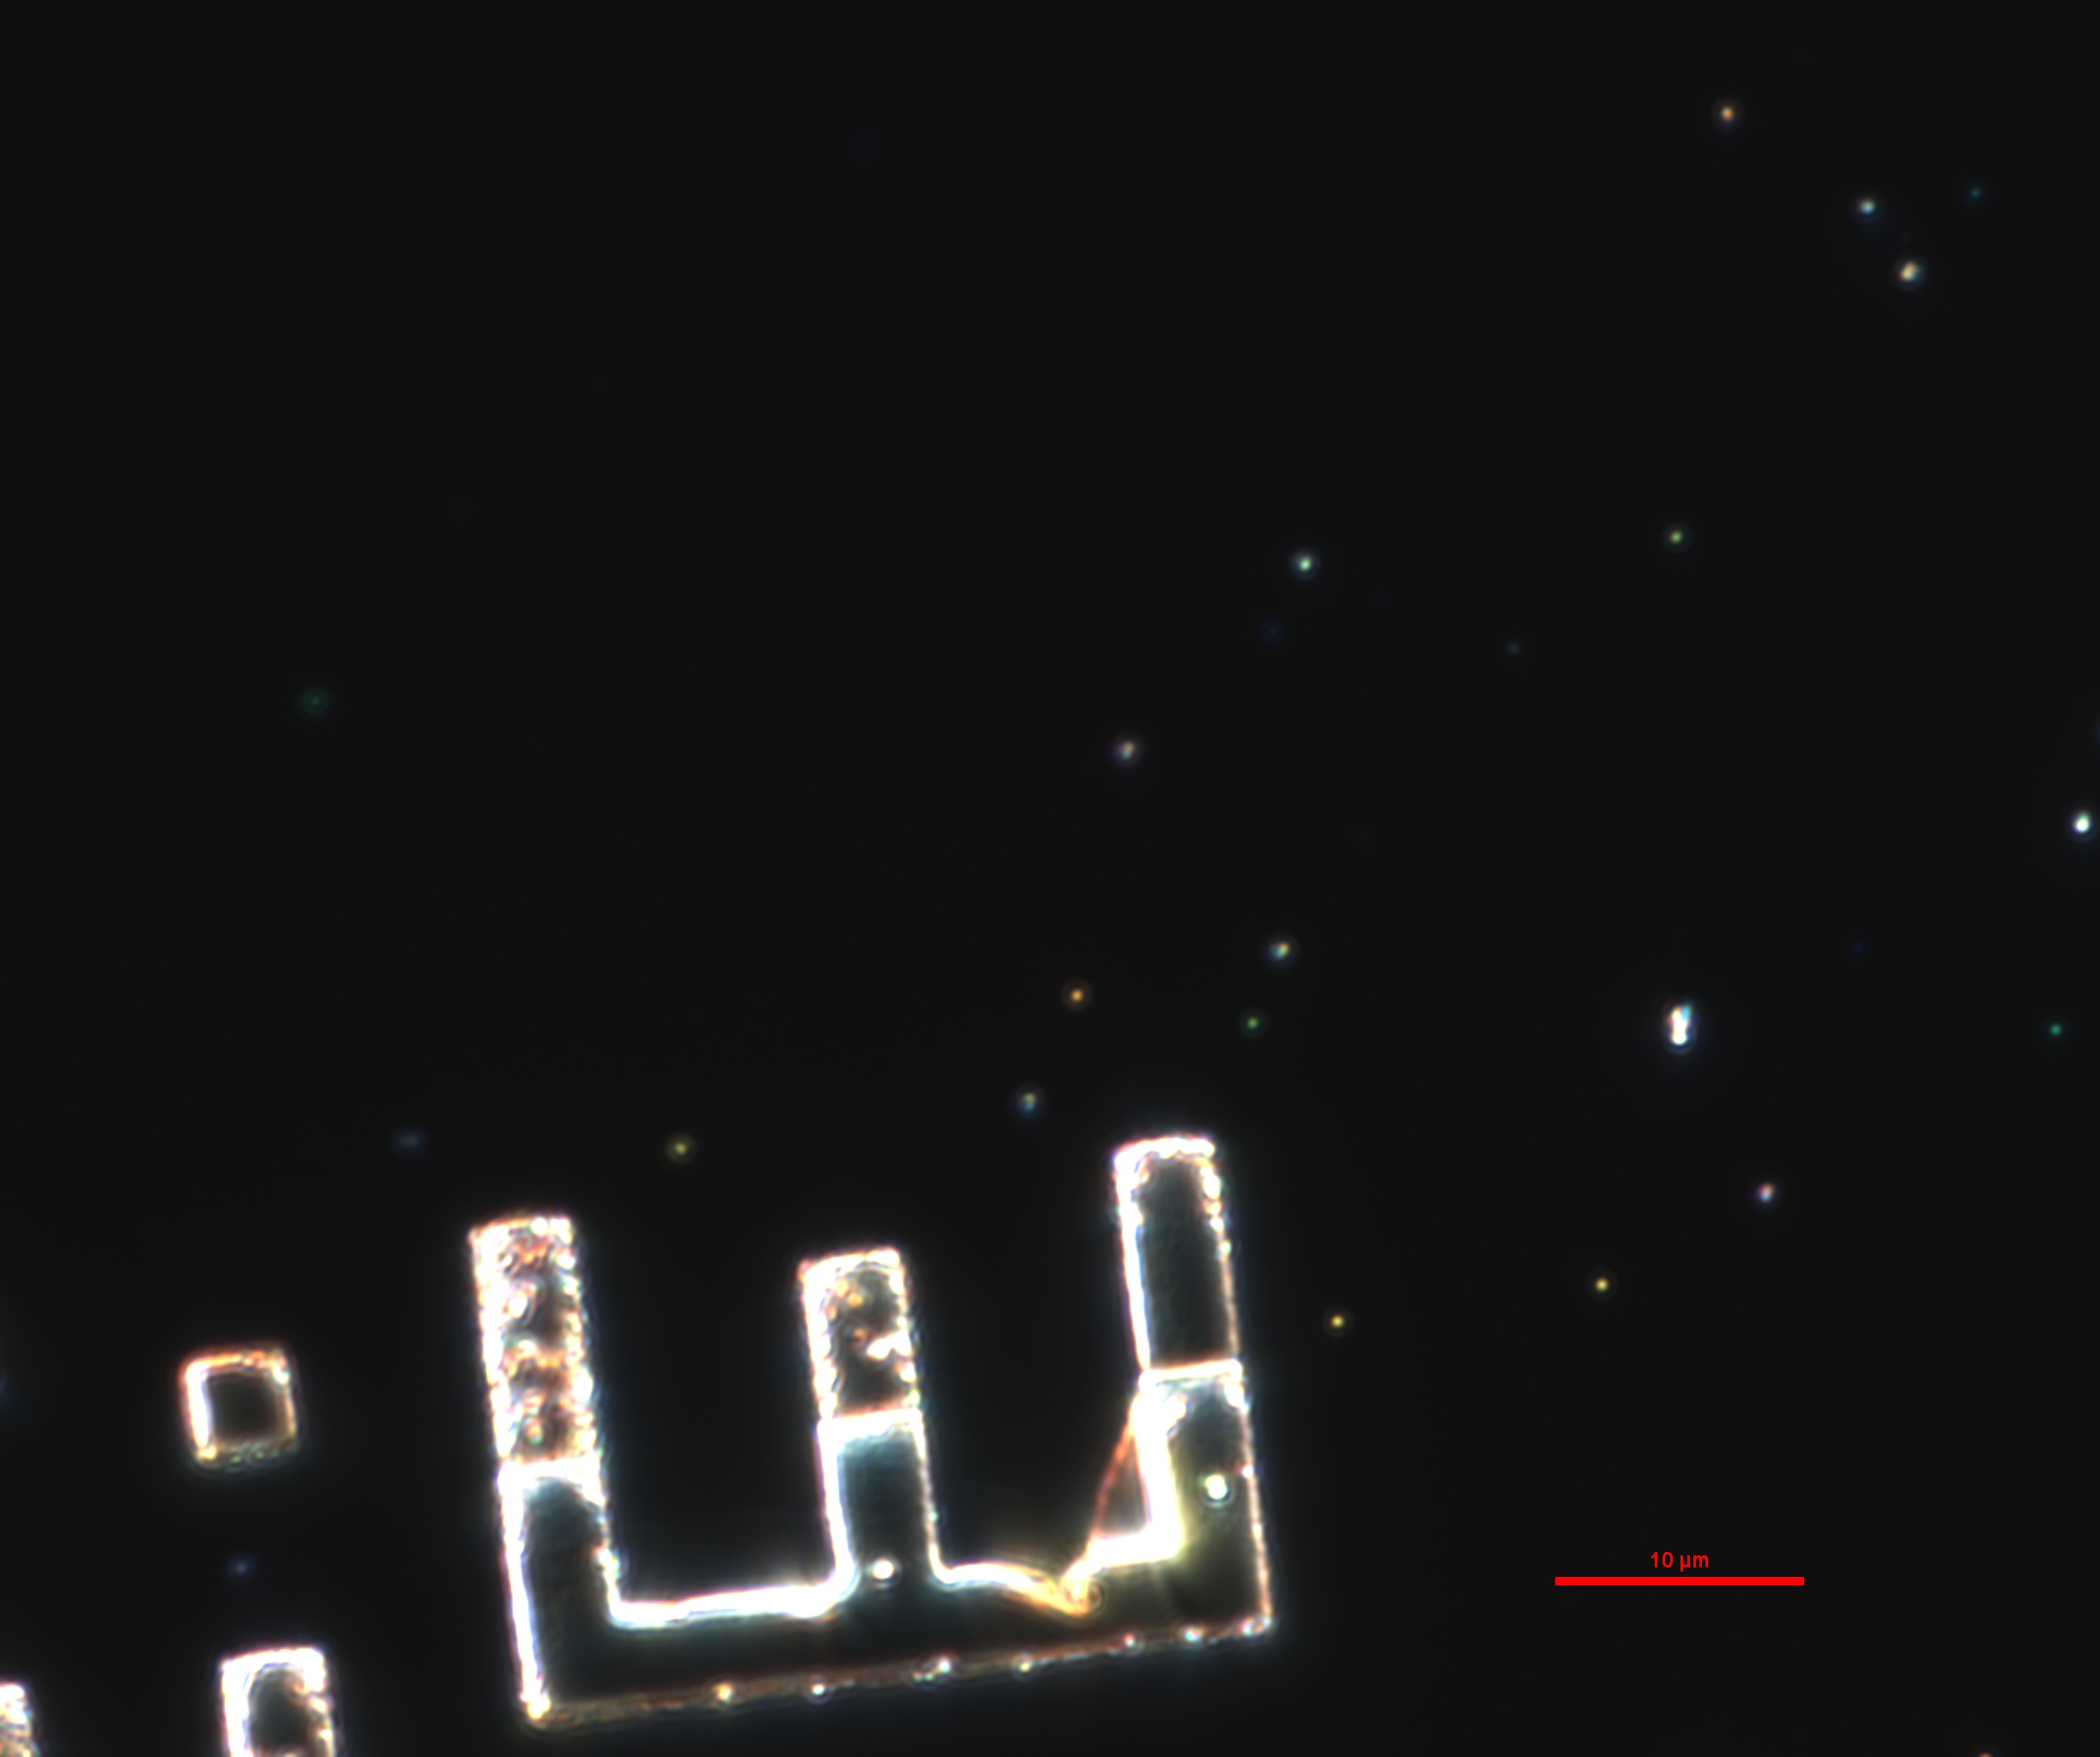
\includegraphics[width=0.4\textwidth, height=0.35\textwidth]{dark_field_ex.png}
    \caption{Dark Field Example}
    \label{fig:dark_field_ex}
\end{figure}
The figure (\ref{fig:dark_field_ex}) show an example of our actual sample viewed through the \textit{dark field} mode. Note that the we have a really high contrast and it possible to clearly recognize each color associated to a specific particle or another object.

Then, to collect our wished spectrum, we have to reduce the detected light thanks to a slit. Thereby, only a few vertical area, with approximately $300 nm$ of width, should be visible by the detector: the \textit{light noise} created by other particles, horizontally next to our studied nanosphere, is avoided. In fact, the computer software parse each horizontal lines in the \textit{extended-}visible range in order to collect the spectrum of this area: if two particles are on the same line, they will be treated as the same entity.
\begin{figure}[h]
    \centering
    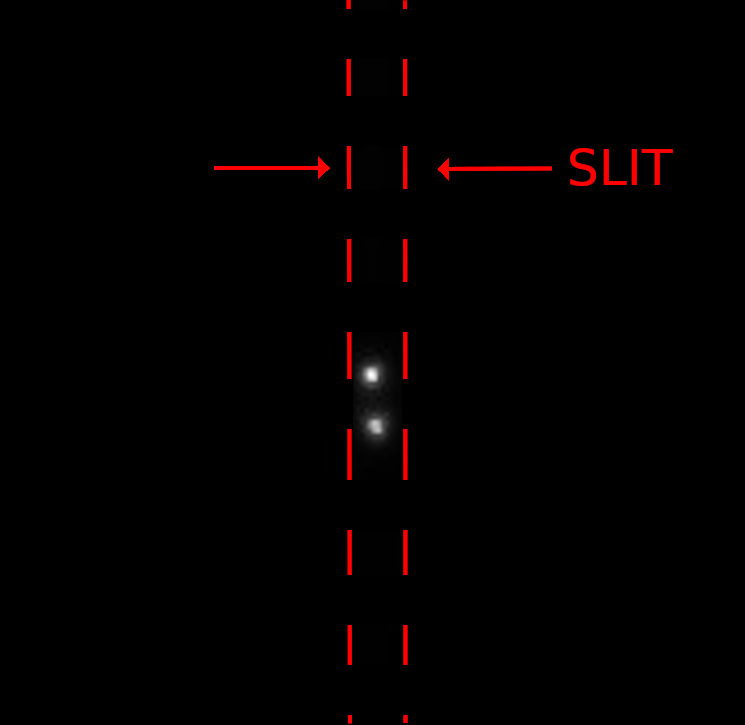
\includegraphics[width=0.4\textwidth, height=0.35\textwidth]{slit_ex.png}
    \caption{Example Of Slit Closed On Two Particles}
    \label{fig:slit_ex}
\end{figure}
Therefore, that is why we put a narrow aperture to the detector, as shown one the previous figure (\ref{fig:slit_ex}).

The first step before actually start our experiment is to numerically calibrate our microscope, that is to say, we have to get some initial data which will be important for computations of the experimental spectrums. In this way, without any incoming light, we save the background spectrum which represents the ambient noise involved by natural emitters like spot lights of the experimental room.
\begin{figure}[h]
    \centering
    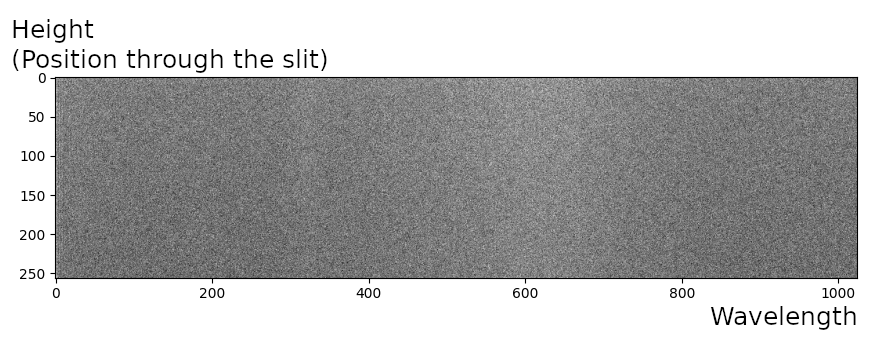
\includegraphics[width=0.45\textwidth, height=0.20\textwidth]{background_ex.png}
    \caption{Example of Background}
    \label{fig:background_ex}
\end{figure}
We could say that these data are collected on a really specific area because of the slit's thickness, but technically, the stored values are really close and only the average is relevant in that case.

In the same way, the incoming light, either in dark or bright field, has a specific distribution (close to a Gaussian one). Thereby, we put a \textit{reference} object as sample on the microscope's repository: a white material involves an exact collected distribution of the incident light.
\begin{figure}[h]
    \centering
    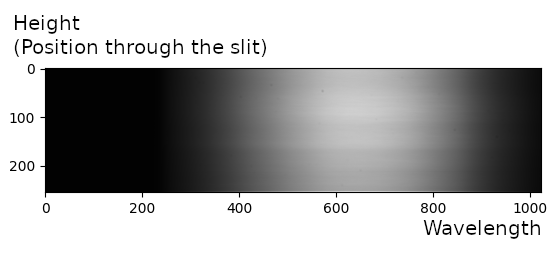
\includegraphics[width=0.45\textwidth, height=0.20\textwidth]{reference_ex.png}
    \caption{Example of Reference}
    \label{fig:reference_ex}
\end{figure}
Note that the area is, here too, really specific, but this homogenous reference object involves the same patch of light distribution whatever the targeted location.

The next step is to get the actual spectrum of our wished nanoparticle. Obviously, because of the dimension of the detected area, we get more than one particle on each image. However, with a clever configuration, we obtain a similar figure from (\ref{fig:raw_data_ex}) after software computations and treatments.
\begin{figure}[h]
    \centering
    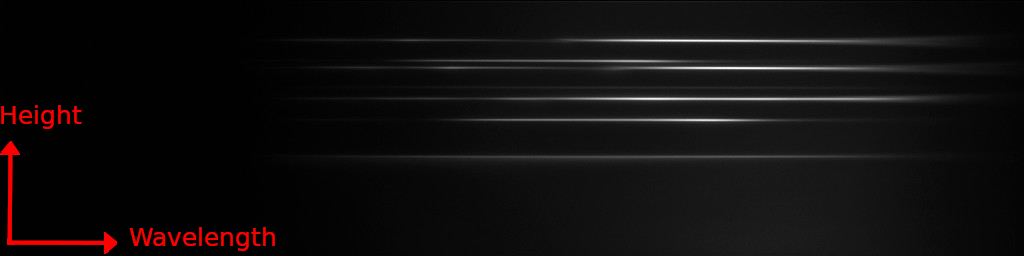
\includegraphics[width=0.45\textwidth, height=0.15\textwidth]{raw_data_ex.png}
    \caption{Raw Data Example}
    \label{fig:raw_data_ex}
\end{figure}
Now, if we extract the line corresponding to our studied particle, we obtain a weird spectrum, pretty close to the following (\ref{fig:spectrum_wout_calc_ex}).
\begin{figure}[h]
    \centering
    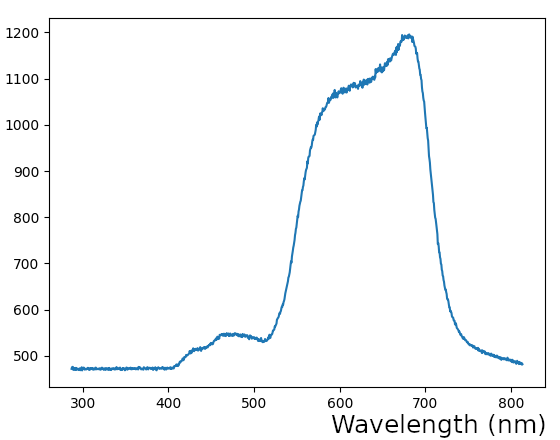
\includegraphics[width=0.4\textwidth, height=0.35\textwidth]{spectrum_wout_calc_ex.png}
    \caption{Spectrum Without (\ref{eq:final_spectrum}) Example}
    \label{fig:spectrum_wout_calc_ex}
\end{figure}
This particular shape, very far from our wished simulation results for nanosphere of silicon, is due to the lack of \textit{background} and \textit{reference} data. In fact, we have to apply this formula for each pixel.
\begin{align}\label{eq:final_spectrum}
FinalSpectrum = \frac{RawSpectrum - Reference}{Background - Reference}
\end{align}
Note that $Background$ is not necessarly a \textit{per pixel} value but could be an average of all pixels stored in \textit{background} as stated previously. Thereby, we obtain the final spectrum, with for instance the figure (\ref{fig:spectrum_w_calc_ex}) from the particle in (\ref{fig:spectrum_wout_calc_ex}).
\begin{figure}[h]
    \centering
    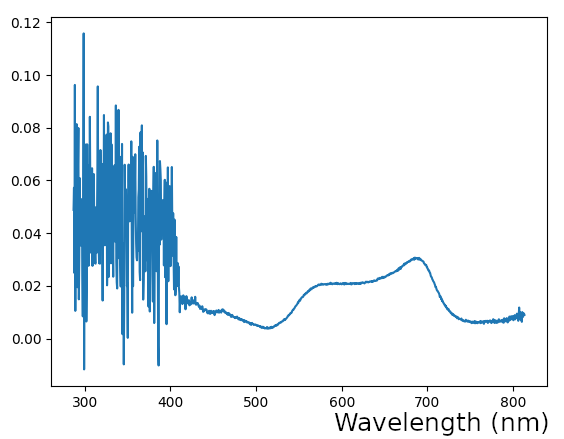
\includegraphics[width=0.4\textwidth, height=0.35\textwidth]{spectrum_w_calc_ex.png}
    \caption{Spectrum With (\ref{eq:final_spectrum}) Example}
    \label{fig:spectrum_w_calc_ex}
\end{figure}
Therefore, this previous result is much more close to our simulation part with two global Mie resonacies and approximately the same shape shifted along the wavelength axis excepted for all values below, approximately, $450 nm$. This last issue is due to the precision of the microscope that is not guaranteed under the visible wavelengths.

\subsection{Atomic Force Microscope}

At this point of the experiment part, we have to couple the spectrum, previously retrieved thanks to the optical microscope, with the size of each studied particle. Thereby, we need another kind of tool in order to detect physically the wished size, that is to say, an instrument able to mesure the diameter, or at least to give an equivalent data, of the desired particle instead of collecting the scattered light intensity. In this way, the best suited tool for this task is the \textit{atomic force microscope}.

The working principle of that kind of microscope is pretty simple. At our \textit{human} scale, the operating mode is roughly similar to the Braille system. Indeed, our sample being totally flat at a macroscopic point of view, the main idea is to drag a tip on the desired experimental surface. This tip is directly connected to a detector collecting the nanometric height variations along the advancement of the last one as shown on figure (\ref{fig:afm_working_principle}). In this way, if the tip runs into a nanoparticle, it could be possible to substract the maximum height to the base one, referencing the surface's sample which is the minimum in that case, in order to get the diameter of the particle (assuming that those are spherical).
\begin{figure}[h]
    \centering
    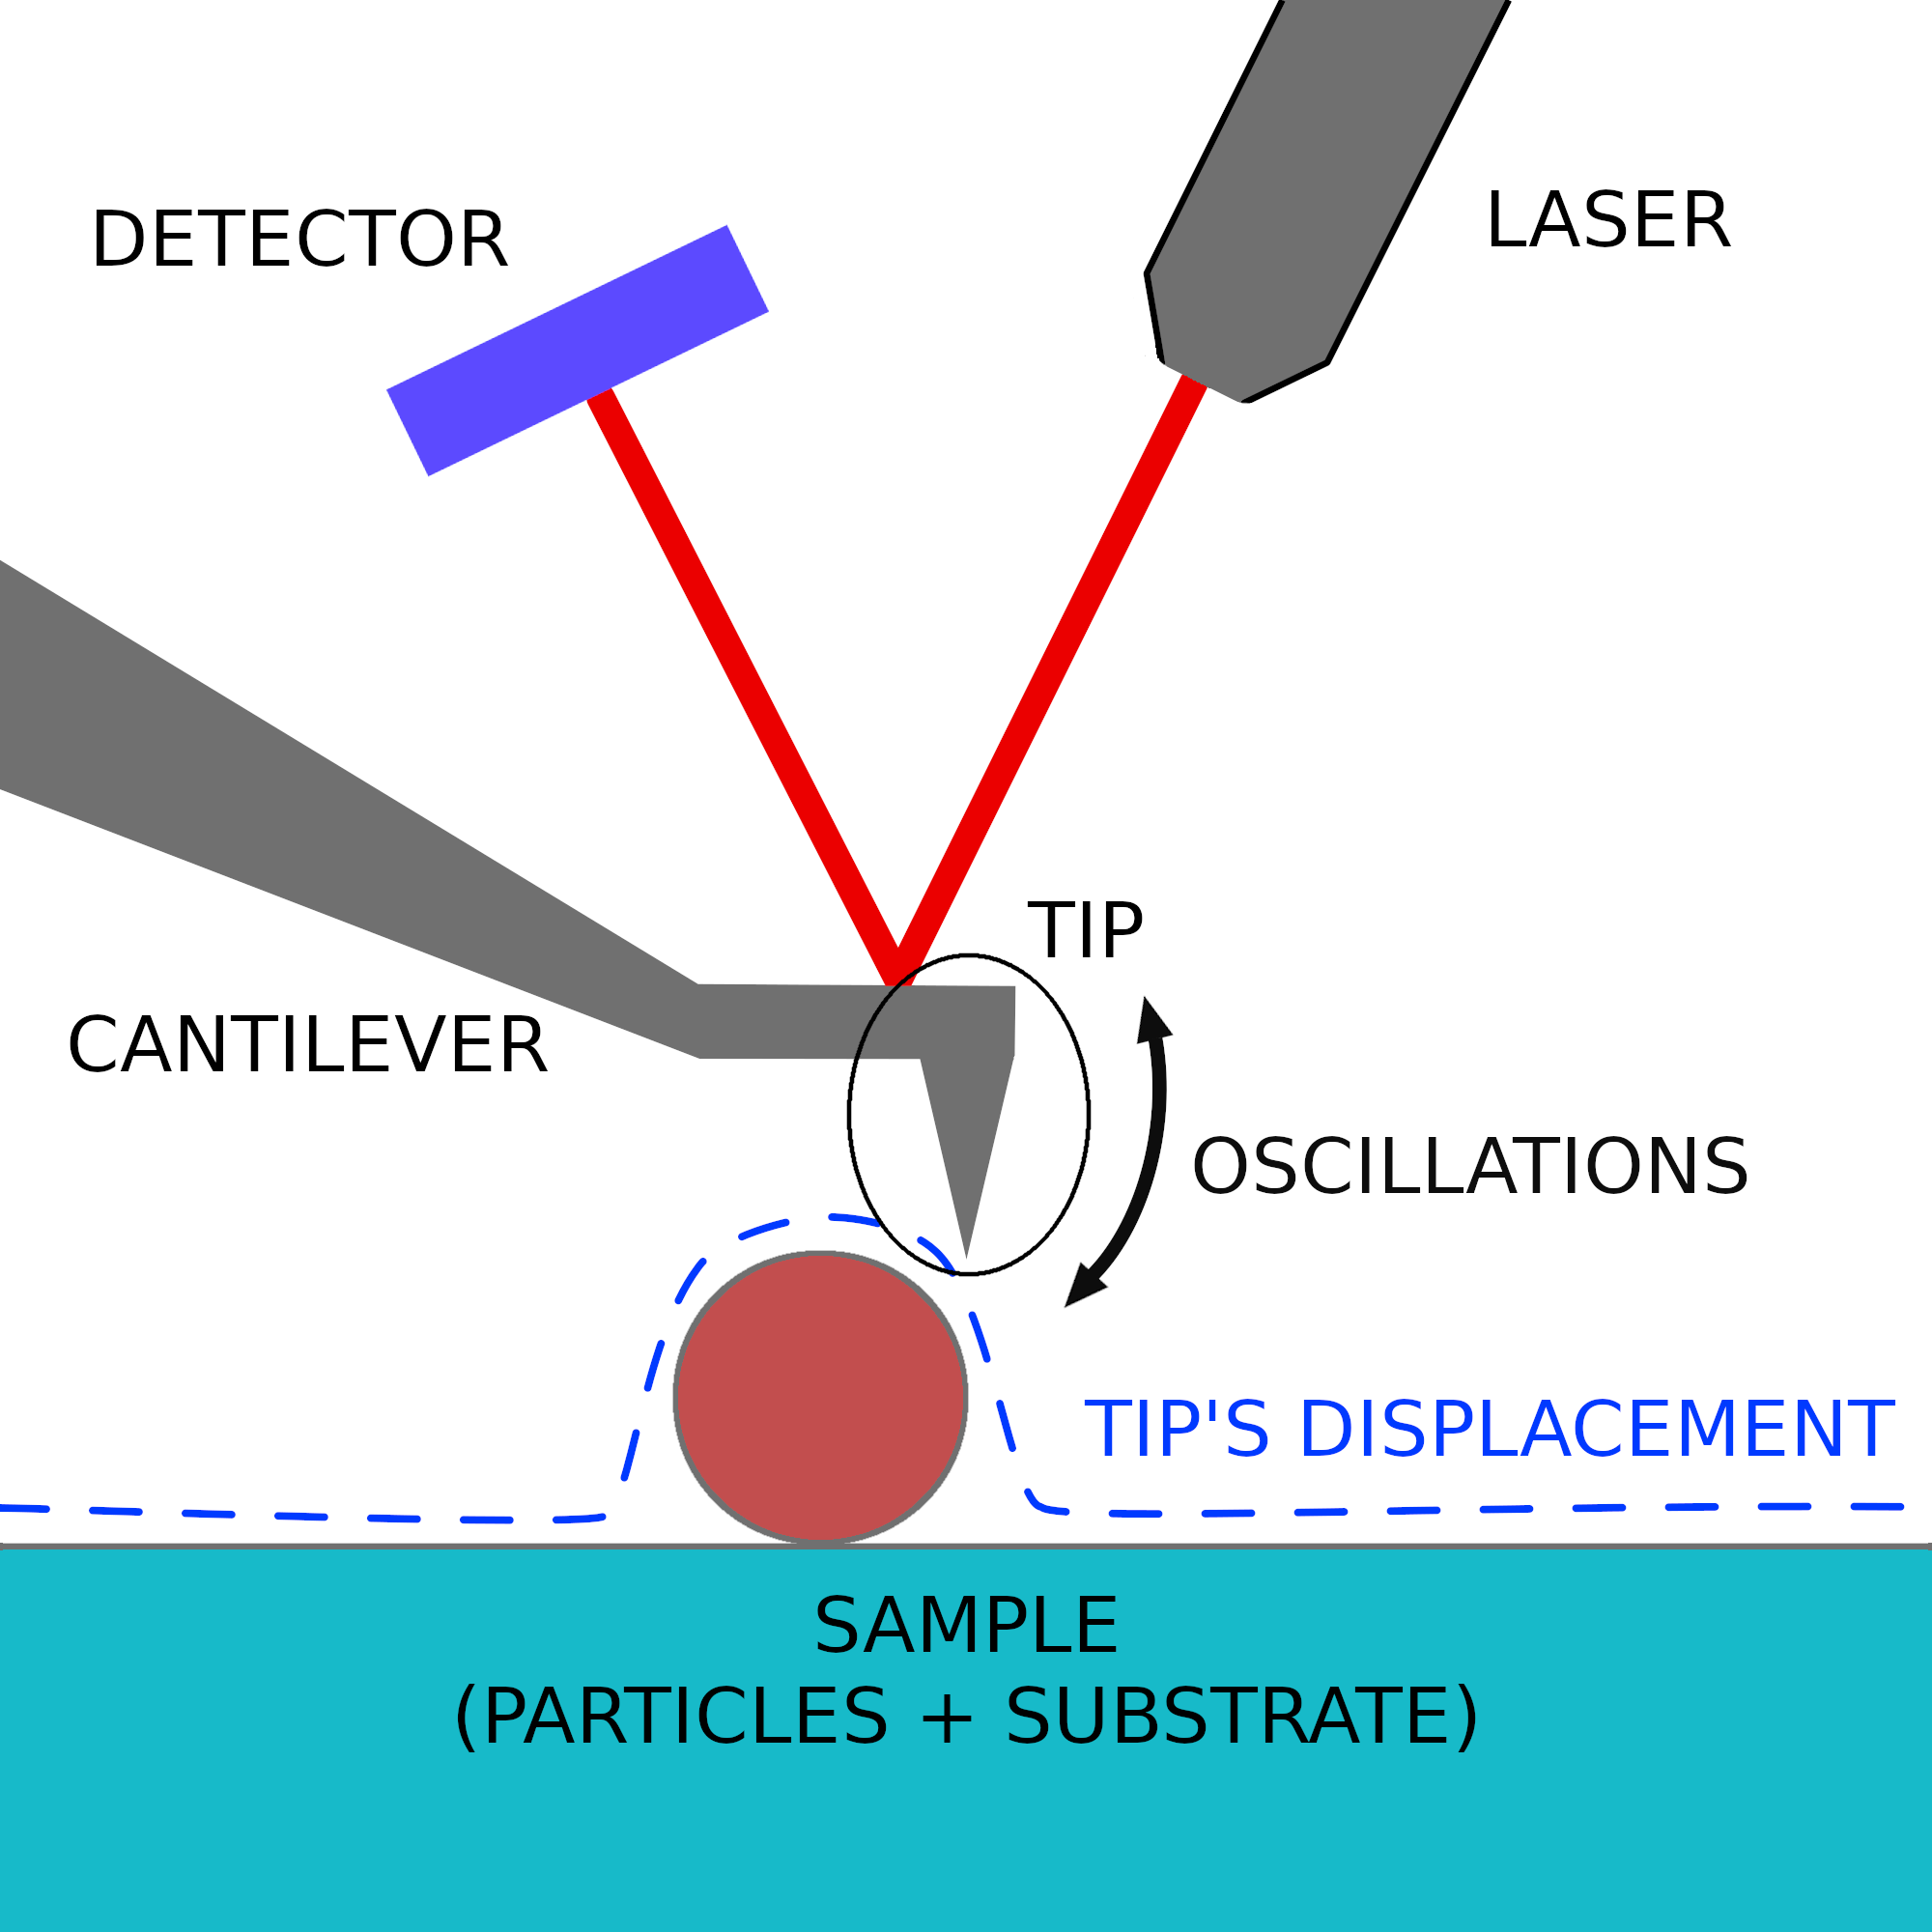
\includegraphics[width=0.4\textwidth, height=0.4\textwidth]{afm_working_principle.png}
    \caption{AFM Working Principle}
    \label{fig:afm_working_principle}
\end{figure}

Technically, even if in general an AFM can use different methods to scan the sample, in our case, the microscope use the \textit{Van der Waals} forces existing between the tip and the nanoparticles. These forces are responsible of the attraction between atoms in a molecule, for instance. Thereby, with no movement, the tip is in balance above the sample without touching it: this is a \textit{non-destructive} scanning tool. The height detector itself is composed of a laser reflecting on the end piece of the cantilever maintaining the tip. When we scan a sample, the tip attached to the cantilever and the laser are moving as a whole block and the tip oscillate around its balance position. In this way, if the tip moves up, compared to its small oscillations, because of a nanoparticle (or another kind of \textit{perturbartion}), the optical way runned by the light, and emitted from the laser, is shorter: we detect a height variation. Effectively, the same process happens when the tip moves down. Then, in order to scan a sample, the tip must move along an arbitrary line and, with a pre-defined length, must shift on the next line to reproduce this task until the quantity of line correspond to the length of these last. Afterward, we obtain a square shaped area of our sample. Moreover, as shown on figure (\ref{fig:afm_scan_dir_config}), multiple scanning modes are available like a double sens scan, that is to say, the tip re-run the scanned line instead of moving out it at the end point, or an horizontal/vertical direction scan, that is to say, the scanned line might be oriented North-South or East-West, and even a start/end point selector, among plenty of other configurations.
\begin{figure}[h]
    \centering
    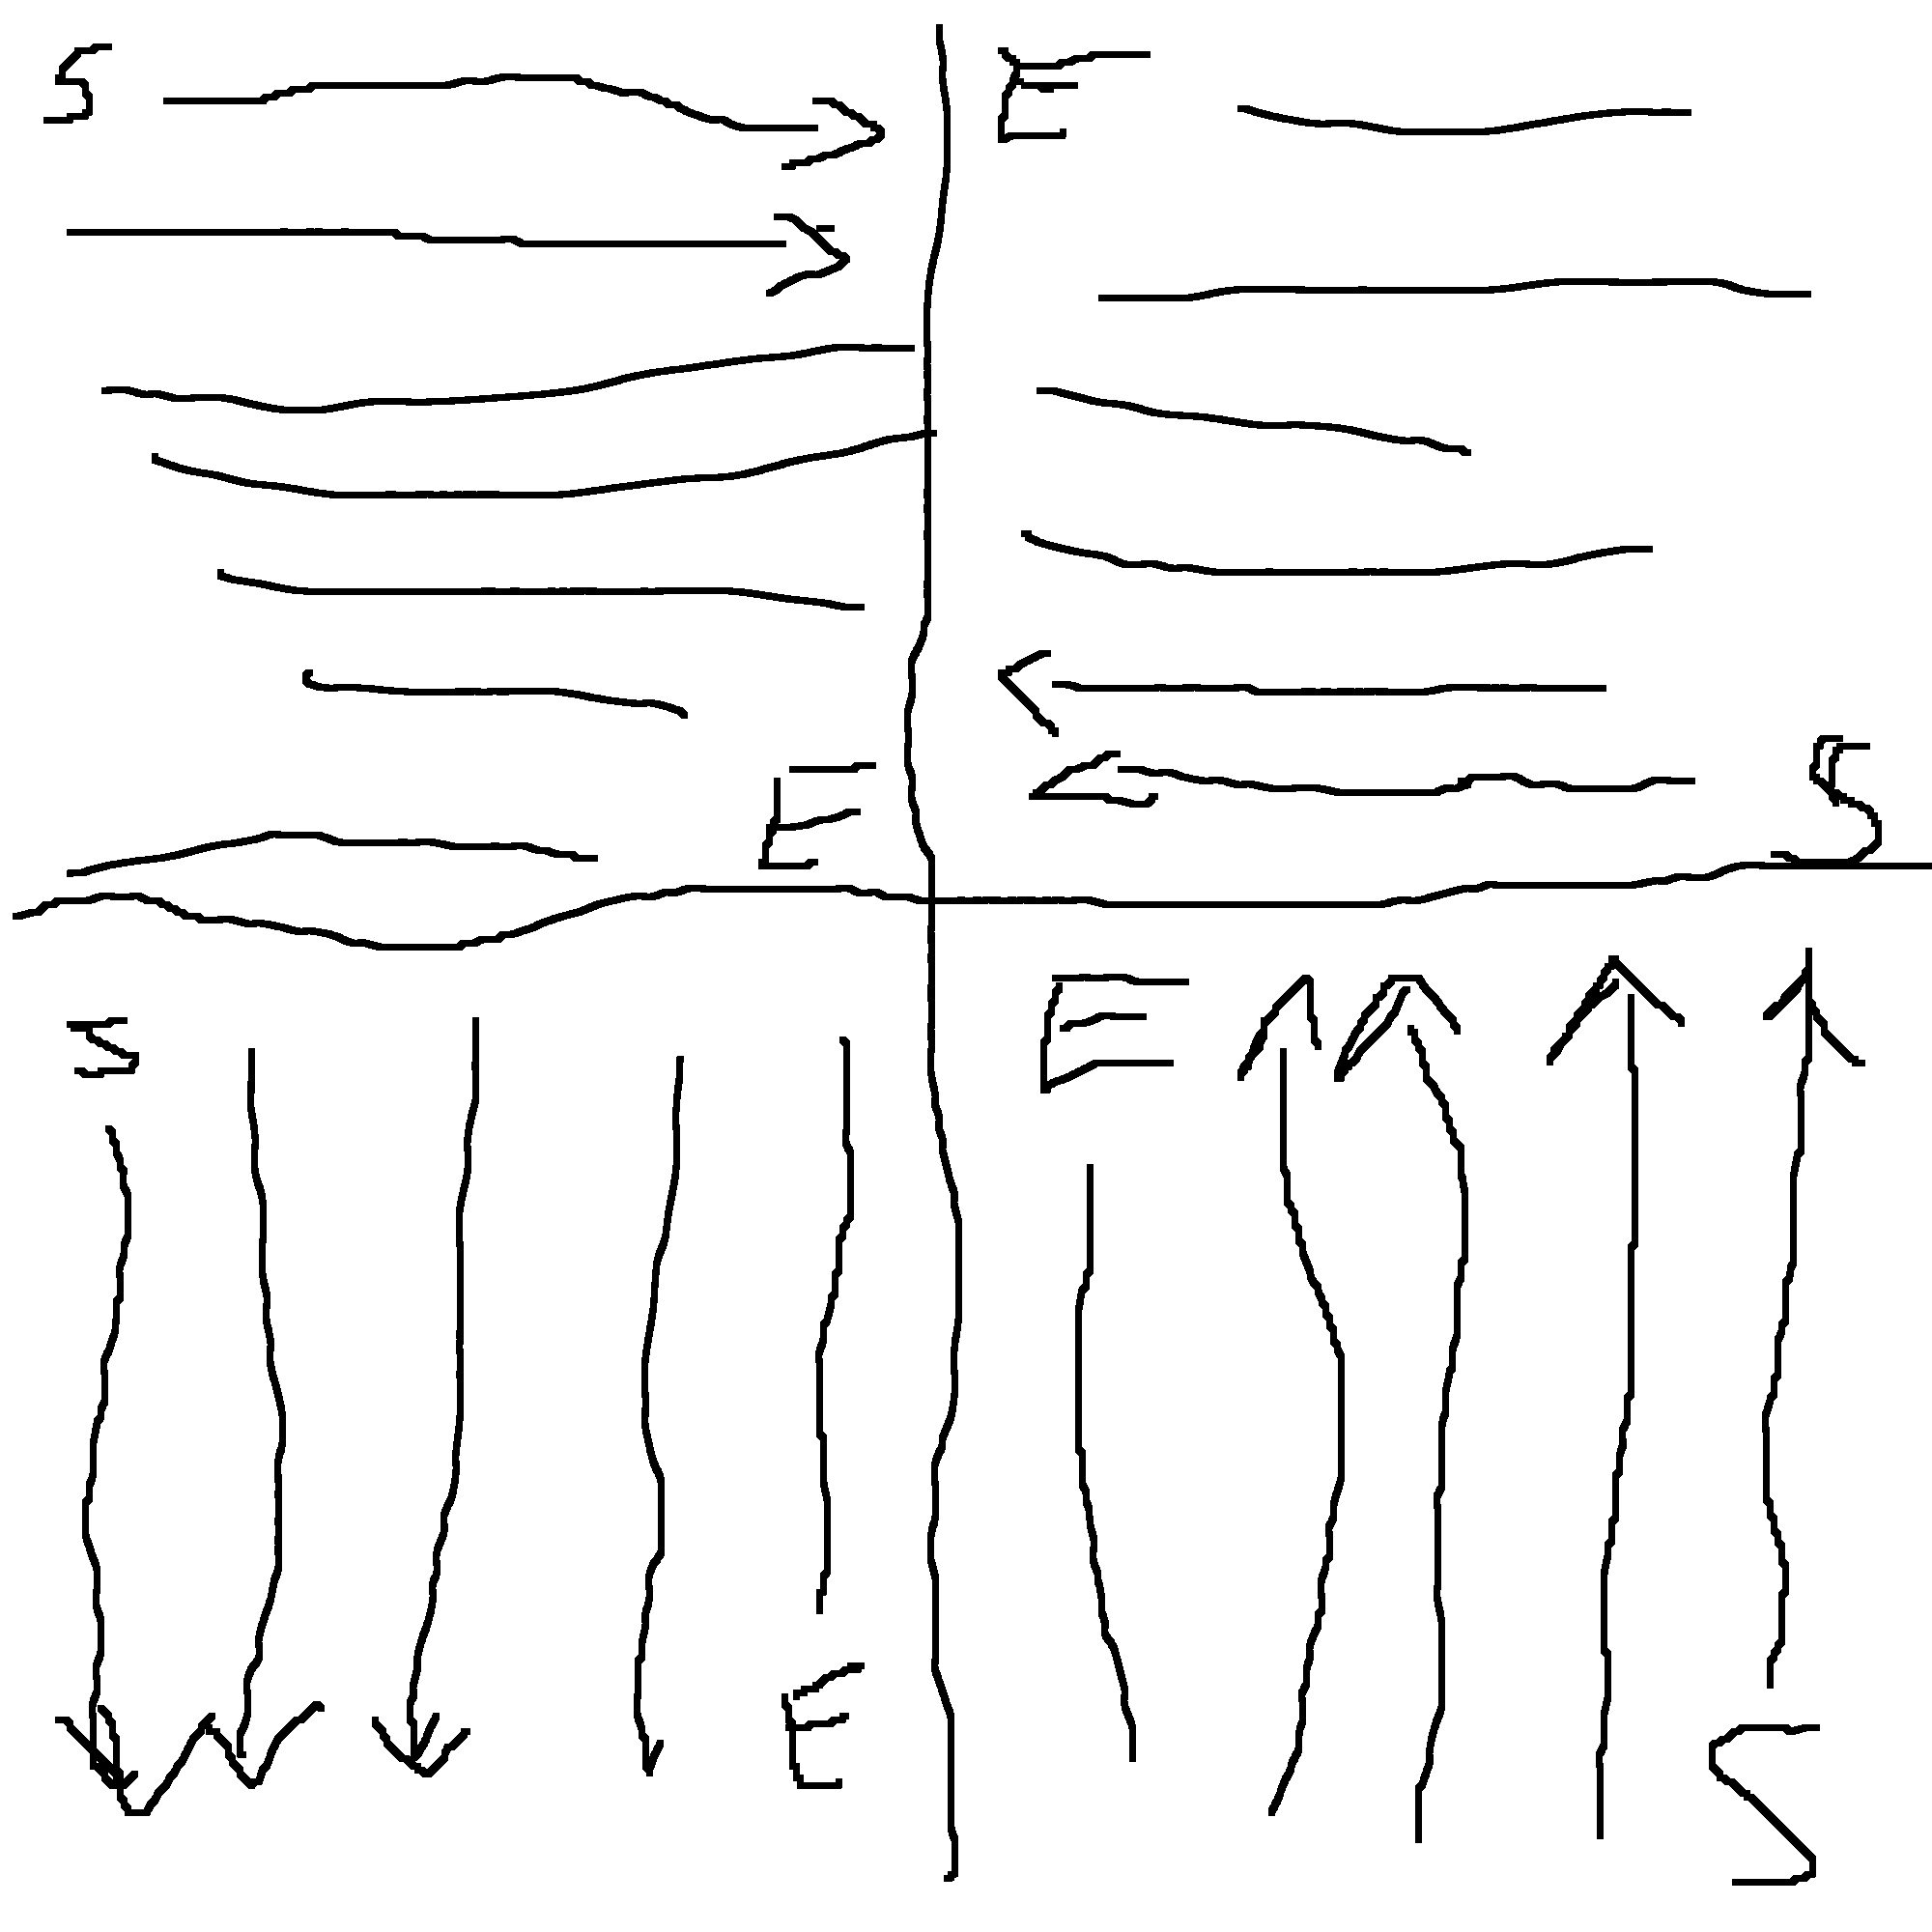
\includegraphics[width=0.4\textwidth, height=0.40\textwidth]{afm_scan_dir_config.png}
    \caption{AFM Direction Configurations (\textit{S} = Start / \textit{E} = End)}
    \label{fig:afm_scan_dir_config}
\end{figure}
Additionaly, as the tip is slightly oscillating around its balance position, it is possible to choose the amount of scanned \textit{points} as shown on figure (\ref{fig:afm_scan_point_config}), that is to say, the number of periods made compared to the advancement of the system (tip, cantilever and laser) corresponding to the amount of generating pixels for a line. 
\begin{figure}[h]
    \centering
    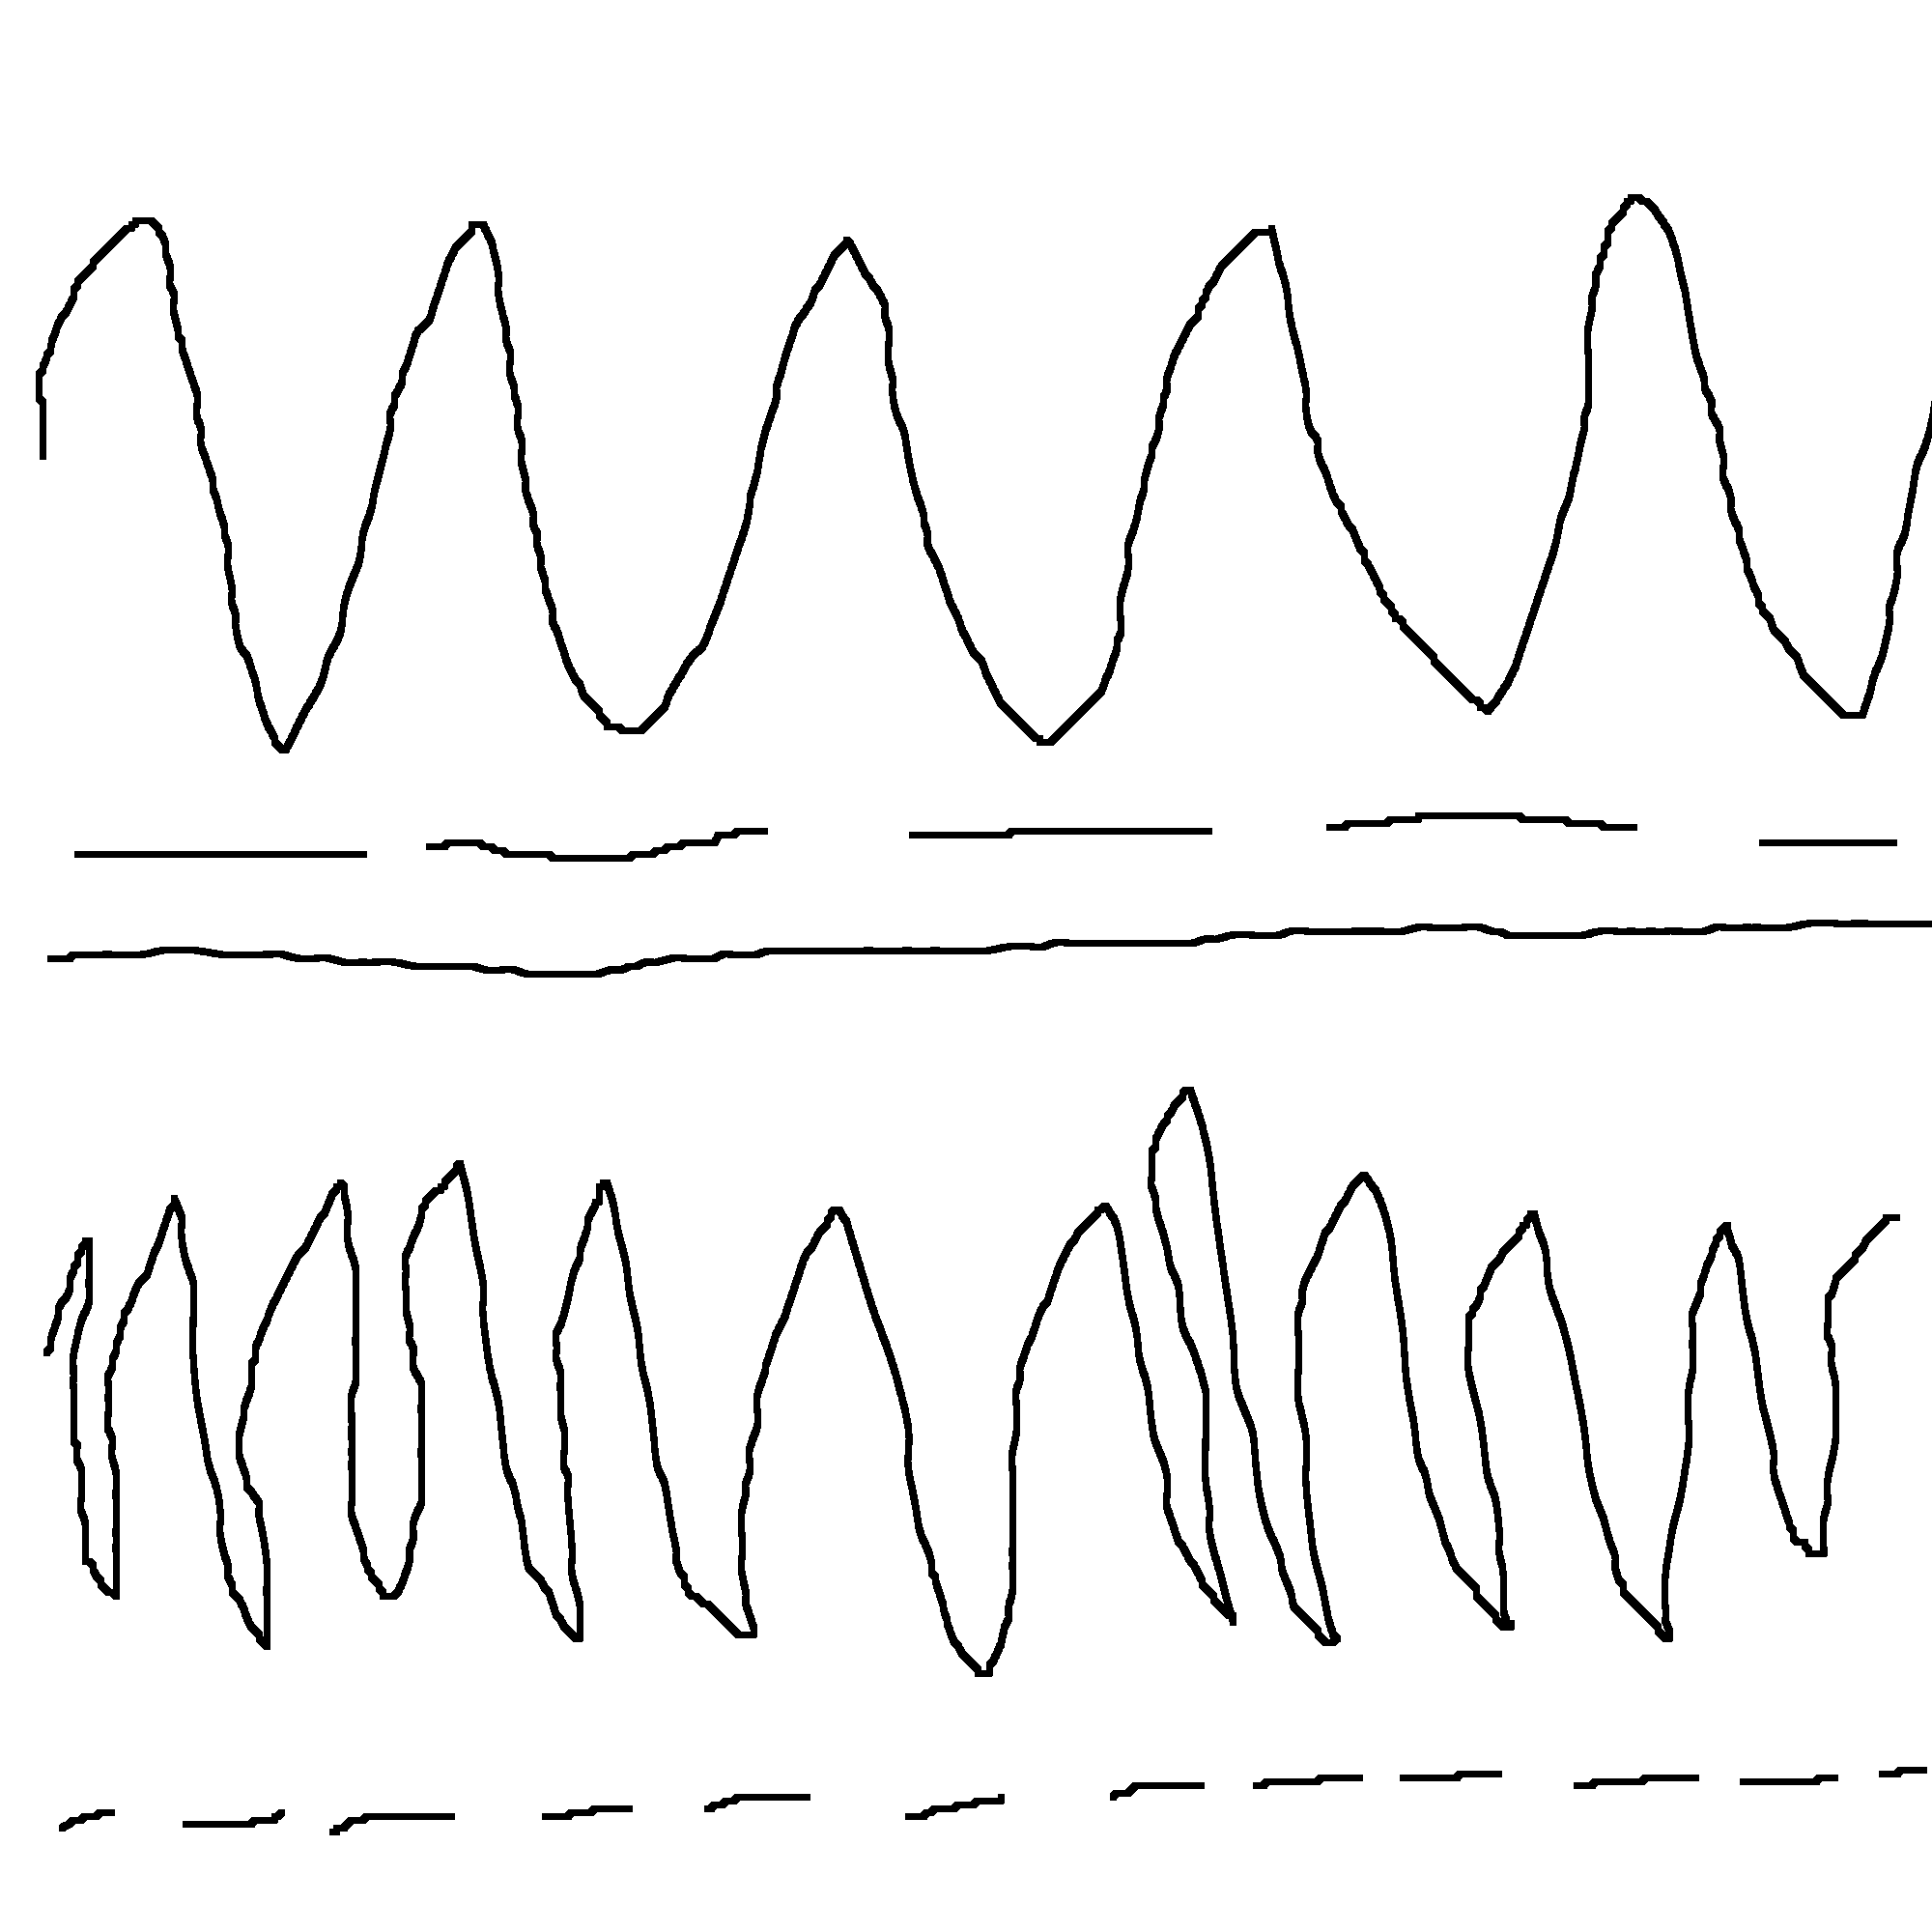
\includegraphics[width=0.4\textwidth, height=0.40\textwidth]{afm_scan_point_config.png}
    \caption{AFM Point Configurations}
    \label{fig:afm_scan_point_config}
\end{figure}
This parameter, associated with the user-defined line's length, might increase or decrease the quality of the collected data. However, increasing the image resolution increases the scanning time by the same. As a rough idea, to scan a $200 \times 200 nm$ square with $100$ points/pixels takes around $10$ minutes whereas, for a $50 \times 50 nm$ area with $256$ points/pixels takes the same amount of time. Therefore, a precise distribution must be adopted between quality, surface and speed in order to collect enough data and retrieve the nanoparticle's size.

In order to illustrate the whole procedure to retrieve the associated size of our studied particle, we will arbitrary choose a nanosphere of silicon as shown on figure (\ref{fig:gwyddion_df_ex}).
\begin{figure}[h]
    \centering
    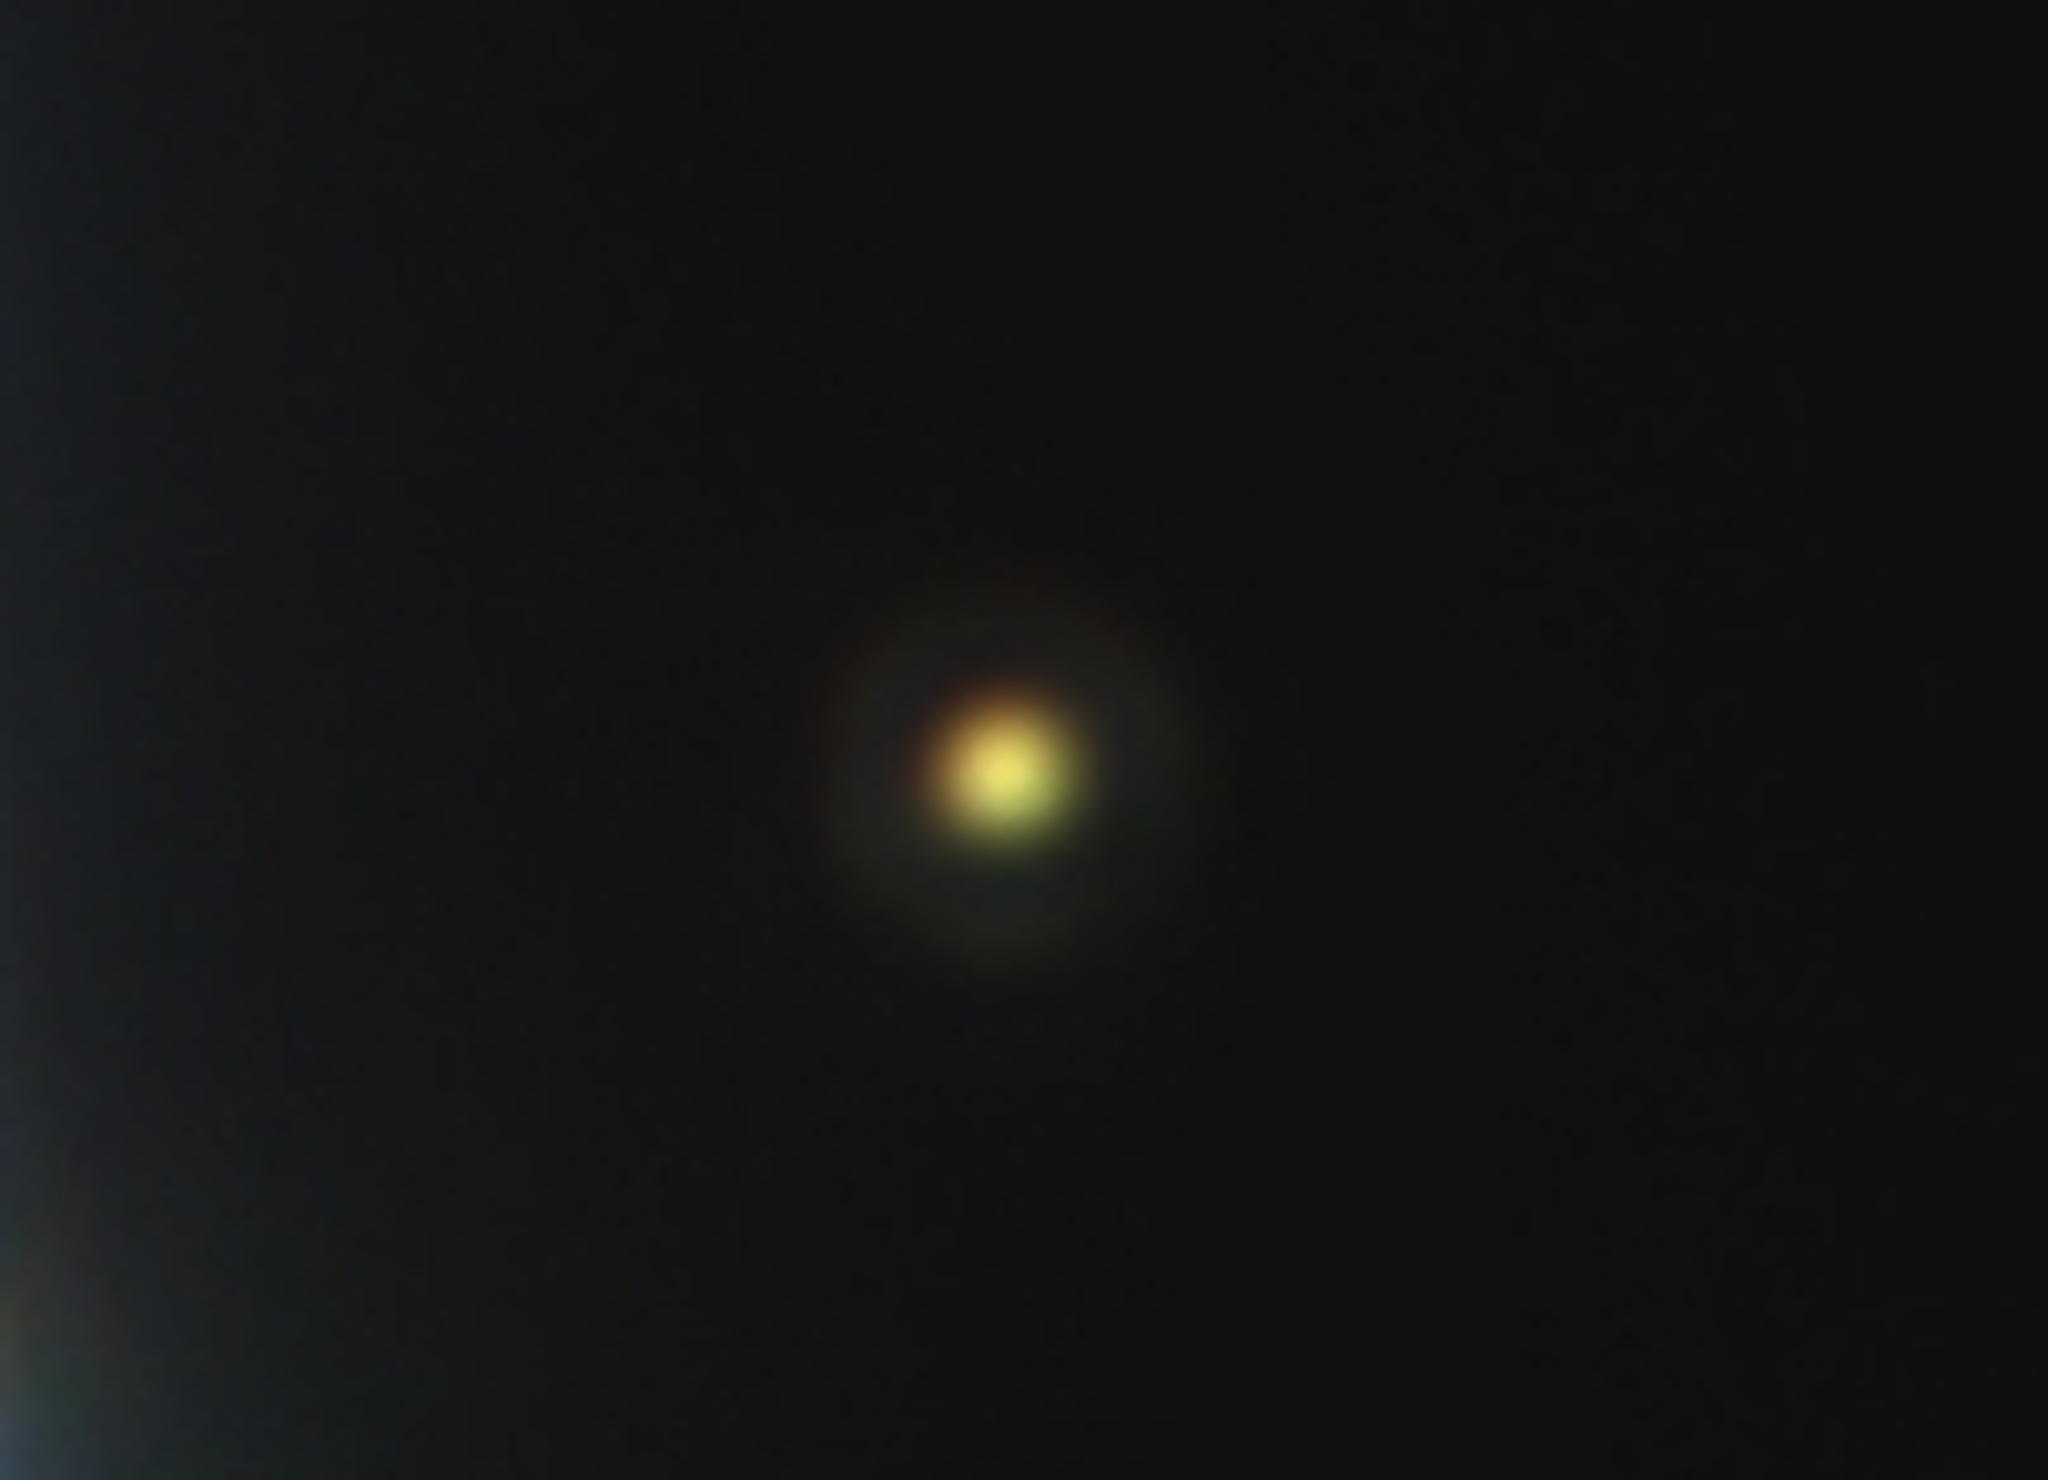
\includegraphics[width=0.4\textwidth, height=0.32\textwidth]{gwyddion_df_ex.png}
    \caption{Example Particle's Image (Dark Field)}
    \label{fig:gwyddion_df_ex}
\end{figure}
At first glance, knowing that a blue scattered light is equivalent to the \textit{smallest} size ($\sim 50 nm$) whereas a red color means the \textit{biggest} one ($\sim 100 nm$), we can easily say that through the yellow-orange color emitted by this particle, we approximate $80 nm$ of radius. However, we need more precision to check our simulation. Thereby, we use the AFM microscope and execute a scan of the targeted area. Unfortunately, for some technical reasons, collecting the final data with enough \textit{quality/pixels} to analyse, requires multiple scan in \textit{low quality} and \textit{large dimension} to locate the right particle. Finally, we obtain the following image (\ref{fig:gwyddion_scan_ex}), through the \textit{Gwyddion} software specialized in AFM data analysis, with a resolution of $256$ \textit{pixels/points} for the line's width.
\begin{figure}[h]
    \centering
    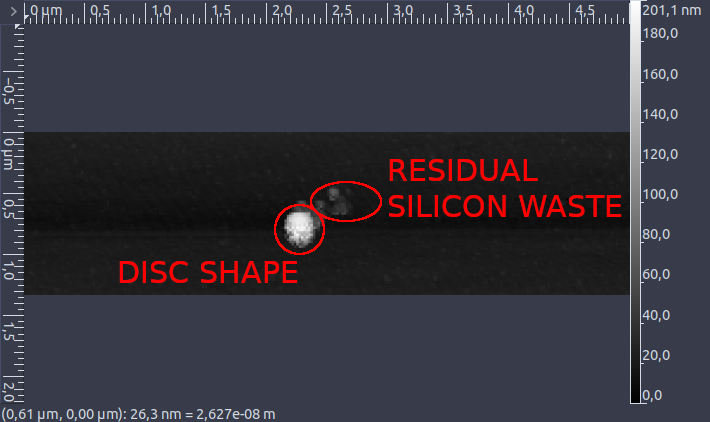
\includegraphics[width=0.4\textwidth, height=0.32\textwidth]{gwyddion_scan_ex.png}
    \caption{Example Particle's Scan}
    \label{fig:gwyddion_scan_ex}
\end{figure}
Note that the scan procedure, started from the bottom side, was aborted when the particle has entirely been scanned: that is why we observe a rectangular area instead of a squared one. Now, it is much more easier to visualize and get the proper data. As we can see, the shape of our particle is close to a disc although some residual silicon \textit{waste} on the North-East side. However this image don't reveal the exact diameter, even if we assume a spherical particle, because of the random pertubration on the edge due to the oscillations of the tip when encountering a particle. In this way, the height, being graduated thanks to a grey-scale put on the right, will give us the maximum of the scan. It is already possible to approximate the diameter as included between $160 nm$ and $190 nm$. Then, we use a tool from the software, exctracting precisely the height scanned along a specific line as shown on figure (\ref{fig:gwyddion_mesure_ex}).
\begin{figure}[h]
    \centering
    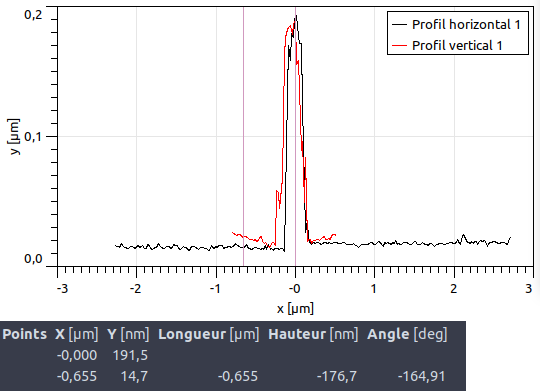
\includegraphics[width=0.4\textwidth, height=0.32\textwidth]{gwyddion_mesure_ex.png}
    \caption{Example Particle's Measurements}
    \label{fig:gwyddion_mesure_ex}
\end{figure}
The exctracted pattern was put on the arbitrary defined top of the particle, that is to say the most white part, producing an horizontal and vertical line in black and red respectively. Therefore, we can differentiate the height between the \textit{flat} area and the maximum in order to retrieve the diameter which is, in this case, $176.7 nm$ giving approximately $88 nm$ and confirm our first hypothesis.

\section{Discussion}

\end{document}